%%%%%%%%%%%%%%%%%%%%%%%%%%%%%%%%%%%%%%%%%%%%%%%%%%%%%%%%%%%%
%%% LIVECOMS ARTICLE TEMPLATE FOR BEST PRACTICES GUIDE
%%% ADAPTED FROM ELIFE ARTICLE TEMPLATE (8/10/2017)
%%%%%%%%%%%%%%%%%%%%%%%%%%%%%%%%%%%%%%%%%%%%%%%%%%%%%%%%%%%%
%%% PREAMBLE
\documentclass[9pt,bestpractices]{livecoms}
% Use the 'onehalfspacing' option for 1.5 line spacing
% Use the 'doublespacing' option for 2.0 line spacing
% Use the 'lineno' option for adding line numbers.
% The 'bestpractices' option for indicates that this is a best practices guide.
% Omit the bestpractices option to remove the marking as a LiveCoMS paper.
% Please note that these options may affect formatting.

\usepackage{lipsum} % Required to insert dummy text
\usepackage[version=4]{mhchem}
\usepackage{siunitx}
\DeclareSIUnit\Molar{M}
\usepackage[italic]{mathastext}
\newcommand{\versionnumber}{0.1}  % you should update the minor version number in preprints and major version number of submissions.
\newcommand{\githubrepository}{\url{https://github.com/MobleyLab/basic_simulation_training}}  %this should be the main github repository for this article
\graphicspath{{figures/}}


%%%%%%%%%%%%%%%%%%%%%%%%%%%%%%%%%%%%%%%%%%%%%%%%%%%%%%%%%%%%%%%%%%%%%
%% Place any additional macros here.  Please use \newcommand* where
%% possible
%%%%%%%%%%%%%%%%%%%%%%%%%%%%%%%%%%%%%%%%%%%%%%%%%%%%%%%%%%%%%%%%%%%%%
\usepackage[colorinlistoftodos]{todonotes}
\usepackage{enumitem} % better handling
\usepackage{pifont} % some unicode-eqsue characters 
\newcommand{\conf}{\mathbf{r}^N}
\newcommand{\peq}{p^{\mathrm{eq}}}


%%%%%%%%%%%%%%%%%%%%%%%%%%%%%%%%%%%%%%%%%%%%%%%%%%%%%%%%%%%%
%%% ARTICLE SETUP
%%%%%%%%%%%%%%%%%%%%%%%%%%%%%%%%%%%%%%%%%%%%%%%%%%%%%%%%%%%%
\title{Best Practices for Foundations in Molecular Simulations : v\versionnumber}

\author[1]{Efrem Braun}
\author[2]{Justin Gilmer}
\author[3]{Heather Mayes}
\author[4]{David L. Mobley}
\author[5]{Jacob I. Monroe}
\author[6]{Samarjeet Prasad}
\author[7]{Daniel M. Zuckerman}
%\author[2\authfn{1}\authfn{4}]{Firstname Initials Surname}
%\author[2*]{Firstname Surname}
\affil[1]{University of California, Berkeley}
\affil[2]{Vanderbilt University}
\affil[3]{University of Michigan}
\affil[4]{University of California, Irvine}
\affil[5]{University of California, Santa Barbara}
\affil[6]{National Institutes of Health}
\affil[7]{Oregon Health and Science University}


\corr{efrem.braun@berkeley.edu }{EB}  % Correspondence emails.  FMS and FS are the appropriate authors initials.
\corr{justin.b.gilmer@vanderbilt.edu}{JG}
\corr{hbmayes@umich.edu}{HM}
\corr{dmobley@mobleylab.org}{DLM}
\corr{jimonroe@umail.ucsb.edu}{JIM}
\corr{p.samar.j@gmail.com}{SP}
\corr{zuckermd@ohsu.edu}{DMZ}

%\contrib[\authfn{1}]{These authors contributed equally to this work}
%\contrib[\authfn{2}]{These authors also contributed equally to this work}

%\presentadd[\authfn{3}]{Department, Institute, Country}
%\presentadd[\authfn{4}]{Department, Institute, Country}

\blurb{This LiveCoMS document is maintained online on GitHub at
\githubrepository; to provide feedback, suggestions, or help improve it, please
visit the GitHub repository and participate via the issue tracker.}

%%%%%%%%%%%%%%%%%%%%%%%%%%%%%%%%%%%%%%%%%%%%%%%%%%%%%%%%%%%%
%%% ARTICLE START
%%%%%%%%%%%%%%%%%%%%%%%%%%%%%%%%%%%%%%%%%%%%%%%%%%%%%%%%%%%%

\begin{document}
\begin{frontmatter}
\maketitle

\begin{abstract}
This document provides a starting point for approaching molecular simulations, guiding beginning practitioners to what issues they need to know about before and while starting their first simulations, and why those issues are so critical. 
This document makes no claims to provide an adequate introduction to the subject on its own. 
Instead, our goal is to help people know what issues are \emph{critical} before beginning, and to provide references to good resources on those topics. 
We also provide a checklist of key issues to consider before and while setting up molecular simulations which may serve as a foundation for other best practices documents.
\end{abstract}
\end{frontmatter}


% List TODOs here
\todototoc
\listoftodos

\section{Introduction}
\label{sec:intro}

Molecular simulation techniques play a very important role in our quest to understand and predict the properties, structure, and function of molecular systems, and are a key tool as we seek to enable predictive molecular design.
Simulation methods are extremely useful for studying the structure and dynamics of complex systems that are too complicated for pen and paper theory and helping interpret experimental data in terms of molecular motions, as well as (increasingly) for quantitative prediction of properties of use in molecular design and other applications.

The basic idea of any molecular simulation method is quite simple; a particle-based description of the system under investigation is constructed and then the system is propagated by either deterministic or probabilistic rules to generate a trajectory describing its evolution over the course of the simulation. 
Relevant properties can be calculated for each ``snapshot'' (a stored configuration of the system, also called a ``frame'') and averaged over the the entire trajectory to compute estimates of desired properties.

Depending on how the system is propagated, molecular simulation methods can be divided into two main categories: Molecular Dynamics (MD) and Monte Carlo (MC).
With MD methods, the equation of motion is numerically integrated and a dynamical trajectory of the system is generated. 
MD simulations can be used for investigating structural, dynamic, and thermodynamic properties of the system.
With MC methods, probabilistic rules are used to generate a new configuration from the present configuration and this process is repeated to generate a sequence of states that can be used to calculate structural and thermodynamic properties but not dynamical properties; indeed, MC simulations lack any concept of time. 
Thus, the ``dynamics'' produced by an MC method are not the temporal dynamics of the system. 
This foundational document will focus on the concepts needed to carry out correct MD simulations that utilize good practices. 
Many, but not all, of the concepts here are also useful for MC simulations and apply there as well, but MC as a whole needs its own document.

Either method can be carried out with different underlying physical theories to describe the particle-based model of the system under investigation.
If a quantum mechanics (QM) description of matter is used, electrons are explicitly represented in the model and interaction energy is calculated by solving the electronic structure of the molecules in the system with no (or few) empirical parameters, but with various approximations to the physics for tractability. 
In a classical description, the molecules are represented by particles representing atoms or groups of atoms.  Each atom may be assigned an electric charge and a potential energy function with a large number of empirical parameters (fitted to experiment, QM, or other data)  is used to calculate non-bonded as well bonded interactions.
Classical simulations are much faster than quantum simulations, making them the methods of choice for vast majority of molecular simulation studies on biomolecular systems in the condensed phase.
%\todo[inline, color={red!20}]{Put in a few-sentence discussion re the size \& timescales of systems and the appropriate method; perhaps like the images often in papers; what are typical sizes and timescales that are tractable? This of course changes with time, but this is a living document so we're good. Also add in general, that the topology does not change--most FF do not allow chemical reactions}

Speed is a particular concern when describing condensed phase systems, as we are often interested in the properties of molecules (even biomacromolecules) in solution, meaning that systems will consist of thousands to hundreds of thousands or millions of atoms.
While system size alone does not require a classical description, if we are interested in calculations of thermodynamic properties like free energy at finite (often laboratory) temperatures, these include substantial entropic contributions (as further discussed below) meaning that fluctuations and correlations of motions within the system affect computed properties, meaning that simulations must not just sample single optimal states but instead must sample the correct distribution of states -- requiring simulations of some length.
Furthermore, many systems of interest, such as polymers (biological and otherwise) have slow motions that must be captured for accurate calculation of properties.
For example, for proteins, relevant timescales span from nanoseconds to seconds or more, and even rearrangements of buried amino acid sidechains can in some cases take microseconds or more, with larger conformational changes and protein folding taking even longer~\cite{Schlick:2010:, Mobley:2012:JComputAidedMolDes}. 
Recent hardware innovations have made microsecond-length simulations for biological systems of 50-100,000 atoms relatively routine, and herculean efforts have pushed the longest simulations out past the millisecond range.
However, the field would like to reach even longer timescales, meaning that switching to a more detailed energy model is only done with some trepidation because slower energy evaluations mean less time available for sampling. 
Thus the need for speed limits the use of quantum mechanical descriptions.

Thus, for the rest of this document we will restrict ourselves to classical MD.

One other important note is that, within classical molecular simulations, bond breaking and forming is generally not allowed (with notable exceptions such as reactive force fields),  meaning that the overall topology or chemistry of a system will remain constant as a function of time.
That is, the particles comprising the system move around, but the chemical identity of each molecule in the system is a constant over the course of the simulation (with only partial exceptions, such as the case of constant pH simulations).
\todo[inline, color={yellow!20}]{DLM: Refs needed here}

Here, we first discuss the scope of this document, then go over some of the fundamental concepts or science topics which provide the underpinnings of molecular simulations, giving references for further reading.
Then, we introduce a variety of basic simulation concepts and terminology, with additional links to further reading.
Our goal is not to cover all topics, but to provide some guidance as to the critical issues which must be considered.

\section{Scope of this document}
\label{sec:scope}

There are several excellent textbooks on classical simulation methods; some we have found particularly helpful are Allen and Tildesley's ``Computer Simulations of Liquids''~\cite{allen_computer_2017}, Leach's ``Molecular Modelling''~\cite{LeachBook}, and Frenkel and Smit's ``Understanding Molecular Simulations''~\cite{Frenkel:2001:}, though there are many other sources.
Tuckerman's ``Statistical Mechanics: Theory and Molecular Simulation''~\cite{Tuckerman:2010:} may be helpful to a more advanced audience.

In principle, anyone with adequate prior knowledge should be able to pick up one of these books and learn the required skills to perform molecular simulations, perhaps with help from a good statistical mechanics and thermodynamics book or two.
In practice, due to the interdisciplinary and somewhat technical nature of this field, many newcomers may find it difficult and time consuming to understand all the methodological issues involved in a simulation study.  
The goal of this document is to introduce a new practitioner to some key basic concepts and bare minimum scientific knowledge required for correct execution of these methods. 
We also provide a basic set of ``best practices'' that can be used to avoid common errors, missteps and confusion in elementary molecular simulations work.
This document is not meant as a full introduction to the area; rather, it is intended to help guide further study, and to provide a foundation for other more specialized best-practices documents focusing on particular simulation areas.

Modern implementations of classical simulations also rely on a large body of knowledge from the fields of computer science and numerical methods, which will
not be covered in detail here.


\section{Science topics}
\label{sec:science}
A variety of fields provide the foundation for our simulation methods and analysis of the data produced by these methods.
A new practitioner does not have to be an expert of all these fields but needs to understand some key concepts from each of these disciplines.
In this section, we survey some topics that we believe even basic users of molecular simulations need to grasp, with suggestions for further reading on these subjects, as a preface for Section~\ref{sec:basics}.
In each subsection, we begin by highlighting some of the critical topics from the corresponding area, then describe what these are and why they are important to molecular simulations.

\subsection{Classical mechanics}
\label{sec:classical_mechanics}
\subsubsection{Key concepts}

Critical concepts from classical mechanics include:
\begin{itemize}
\item Newton's equations of motion and constants of motion
\item Hamilton's equations
\item Point particles and rigid bodies
\item Holonomic constraints
\end{itemize}

Molecular simulation methods work on many particle systems following the rules of classical mechanics. 
Basic knowledge of key concepts of classical mechanics is important for understanding simulation methods.
Here, we will assume you are already familiar with Newtonian mechanics.

Classical molecular models typically consist of point particles carrying mass and electric charge, as well as potentially additional interactions such as van der Waals interactions and bonded interactions of various types.
Sometimes it is much more efficient to freeze the internal degrees of freedoms and treat the molecule as a rigid body where the particles do not change their relative orientation as the whole body moves; this is commonly done, for example, for rigid models of the water molecule.
Due to the high frequency of the O-H vibrations, accurately treating water classically would require a very small time step, so for computational efficiency water is often instead treated as a rigid body.
Keeping specified objects rigid in a simulation involves applying holonomic constraints, where the rigidity is defined by imposing a minimal set of fixed bond lengths and angles through iterative procedures during the numerical integration of the equation of motion (see Section~\ref{sec:integrators} for more on constraints and integrators).
It is important to understand the concept of point particles, rigid bodies and constraints.

Classical mechanics has several mathematical formulations --- namely the Newtonian, Hamiltonian and Lagrangian formulations.
These formulations are equivalent, but for certain applications one formulation can be more appropriate than the other. 
Many simulation methods use the Hamiltonian formulation and therefore basic knowledge of Hamiltonian mechanics is essential if you wish to understand the details of simulation methods.

Classical mechanics has several conserved quantities and simulators should be familiar with these, for example, the total energy of a system is a constant of motion.
These concepts play very important role in development and proper implementation of simulation methods.
For example, a particularly straightforward check of the correctness of an MD code is to test the quality of the energy conservation.

Most books on molecular simulations have a short discussions or appendices on classical mechanics that can serve the purpose of very quick introductions to the basic concepts; Shell's book also has a chapter on simulation methods which covers some of these details~\cite{ShellBook}.
A variety of good books on classical mechanics are also available and give further details on these concepts.

\subsection{Thermodynamics}
\label{sec:thermodynamics}

\subsubsection{Key concepts}
A variety of thermodynamic concepts are particularly important for molecular simulations:
\begin{itemize}
\item Temperature, pressure, stress
\item Internal energy, enthalpy
\item Gibbs and Helmholtz free energy
\item Entropy
\end{itemize}

One of the main objectives of molecular simulations is to estimate/predict thermodynamic behavior of real systems as observed in the laboratory.
Typically this means we are interested in macroscopic systems, consisting of $10^23$ particles or more (i.e. at least several moles of particles). 
But properties of interest include not only macroscopic, bulk thermodynamic properties, such as density or heat capacity,
but also microscopic properties like specific free energy differences associated with, say, changes in the conformation of a molecule.
For this reason, it is important to understand key concepts in thermodynamics, such as temperature, pressure, entropy, internal energy, various forms of free energy, and the relationships between them.
Paramount, however, is an understanding of the connection between thermodynamics and statistical mechanics, which allows us to relate macroscopic, experimental measurements to the behavior of the much smaller system that is simulated.
This topic involves a variety of subtleties and thus can be a confusing and difficult, so we refer the reader to a more extensive discussion in one of several books~\cite{ShellBook, DillBook}.

As an example, consider temperature.
In a macroscopic sense, we understand this quantity very intuitively as how hot or cold something is.
The laws of thermodynamics provide us with a further abstraction, telling us that this is in fact the derivative of the internal energy with respect to the entropy.
This mathematical definition itself is not particularly helpful, but provides a starting point for other derivations.
If we want to understand temperature from the point of view of understanding molecular behavior, we finally must turn to statistical mechanics.
Since molecular dynamics is mostly used to simulate behavior at the molecular or atomistic level, it is necessary to utilize statistical-mechanical expressions in computing what would be observed as the macroscopic, thermodynamic temperature.

This discussion should not provide the impression that statistical mechanics is more important than thermodynamics.
The two are intimately connected and we must rely on both to successfully conduct and obtain information from MD simulations.
In particular, thermodynamics provides rigid rules that must be satisfied if we are to faithfully reproduce reality.
For instance, if energy is not conserved, the first law is not satisfied and we are for sure simulating a system out of equilibrium (i.e. we are somehow adding or removing energy).
In this sense, the laws of thermodynamics provide us rigorous sanity checks in addition to many useful mathematical relations for computing properties.
Basic thermodynamic principles thus also dictate proper simulation protocols and associated best practices.

The concept of the thermodynamic limit is particularly important.
Specifically, as the size of a finite system is increased, keeping the particle number density roughly constant, at some point it is said to reach the thermodynamic limit where its behavior is bulk-like and no longer depends on the extent of the system.
Thus, small systems will exhibit unique behaviors that reflect their microscopic size, but sufficient large systems are said to have reached the thermodynamic limit and macroscopic thermodynamics applied.

Although we usually think of thermodynamics applying macroscopically and statistical mechanics applying on the microsopic level, it is important to remember that the laws of thermodynamics still hold \textit{on average} regardless of the length scale.
That is, a molecule in contact with a thermal bath will exchange energy with the bath, but its average energy is a well-defined constant.
This allows us to define thermodynamic quantities associated with microscopic events, such as the binding of a ligand to a protein.
This is of course useful because it allows us to assign molecular meaning to a well-defined thermodynamic processes that can only be indirectly probed by experiment.
Importantly, as long as we have carefully defined our ensemble and thermodynamic path, we can apply the powerful relationships of thermodynamics to more easily calculate many properties of interest.
For instance, one may use molecular dynamics to efficiently numerically integrate the Clapeyron equation and construct equations of state along phase coexistence curves~\cite{Kofke1993, GonzalezSalgado2010}.

\todo[inline, color={green!20}]{JIM: I also want to mention that some thermodynamic properties are only truly well-defined for many molecules, not for single molecules or isolated molecules. This is a tricky discussion, though. DLM: What did you have in mind? } 

\subsubsection{Books}
Equilibrium thermodynamics is taught in most undergraduate programs in physics, chemistry, biochemistry and various engineering disciplines.
Depending on the background, the practitioner can choose one or more of the following books to either learn or refresh their basic knowledge of thermodynamics. 
Here are some works we find particularly helpful:
\begin{itemize}
\item Atkins and De Paula's ``Physical Chemistry'' \cite{AtkinsBook}, chapters 1 to 4.
\item McQuarrie and Simon's extensive work, ``Physical Chemistry: A Molecular Approach''~\cite{McQuarrie:1997:}
\item Dill's ``Molecular Driving Forces''~\cite{DillBook}
\item Kittel and Kroemer's ``Thermal Physics''~\cite{Kittel:1980:}
\item Shell \cite{ShellBook}: Chapters 1-15.
\end{itemize}


\subsection{Classical statistical mechanics}
\label{sec:stat_mech}
\subsubsection{Key concepts}
Key concepts from statistical mechanics are particularly important and prevalent in molecular simulations:
\begin{itemize}
\item Ensembles, distribution functions for different ensembles. Equivalence of ensembles
\item What equilibrium means and the difference between equilibrium and non-equilibrium.
    For instance, what is usually called an ``equilibrium trajectory'' generally will not embody a good sample of the equilibrium ensemble due to insufficient sampling.  
        On the other hand, truly non-equilibrium conditions such as driven transitions and relaxation are fundamentally different. 
        Note that relaxation can occur to the equilibrium ensemble or a non-equilibrium condition (e.g., steady state).
\item Clarify differences between nonequilibrium ensembles: driven
    nonequilibrium steady-state, systems driven out of equilibrium by a time-dependent field, systems initially out of equilibrium but relaxing
        to equilibrium
\item Time averages and ensemble averages
\item Fluctuations
\item Correlation functions
\end{itemize}
\todo[inline, color={yellow!20}]{DLM: This list is bothering me because it is longer than the others, has more statements in it, and doesn't totally connect with what's in this section. Not sure what to do with it.}

Traditional discussions of classical statistical mechanics, especially concise ones, tend to focus first or primarily on macroscopic thermodynamics and microscopic \emph{equilibrium} behavior based on the Boltzmann factor, which tells us that configurations $\conf$ occur with (relative) probability $\exp[-U(\conf)/k_B T]$, based on potential energy function $U$ and temperature $T$ in Kelvin units.  
Dynamical phenomena and their connection to equilibrium tend to be treated later in discussion, if at all.  
But in both fundamental and practical ways, this ordering is wrong.  
Think Arrhenius first, then Boltzmann.

MD simulation, like nature itself, runs dynamics.  
Any equilibrium phenomena may (or may not) occur as a consequence and equilibrium behavior is hardly automatic~\cite{Zuckerman:2010:}.  
In fact, based on current and foreseeable computational technology, it is much safer to assume that your simulation will not exhibit equilibrium behavior.  
However, an MD simulation is guaranteed to exhibit dynamical behavior.

\begin{figure}[h]
\centering
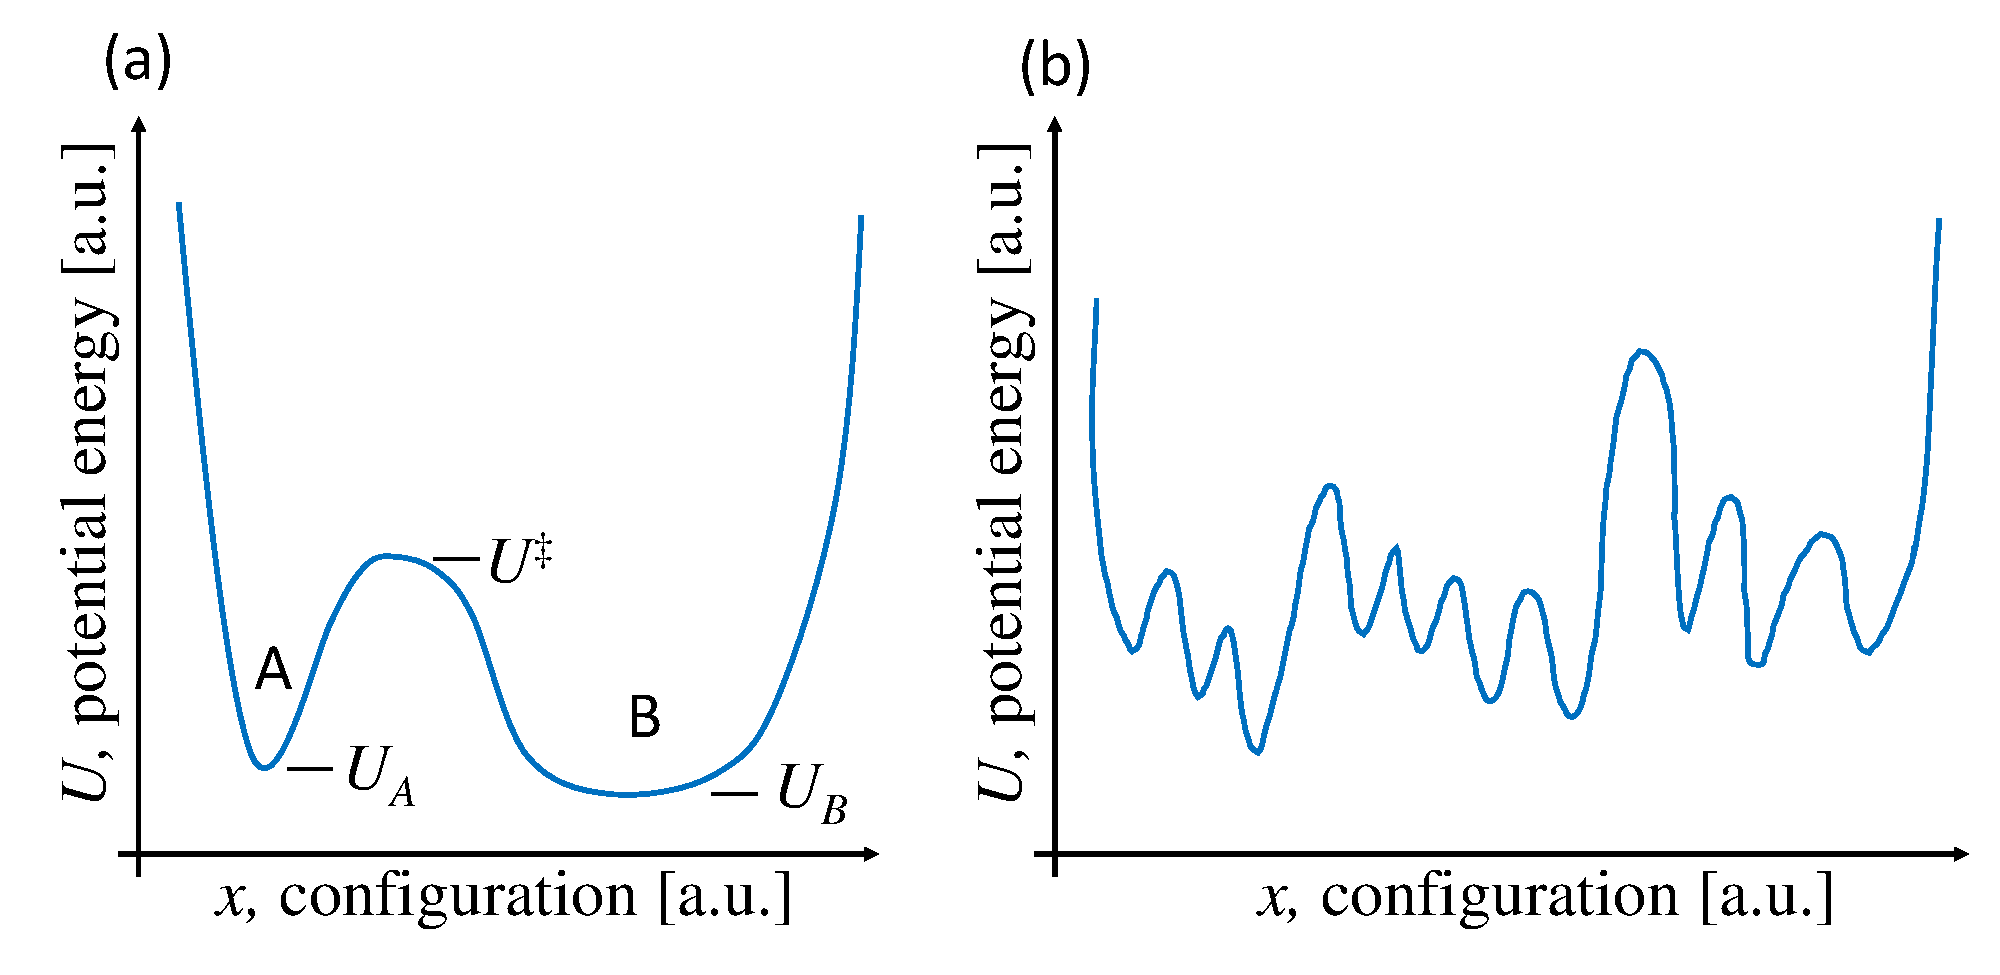
\includegraphics[width=\linewidth]{simplelandscapes.pdf}
\caption{Energy landscapes.  (a) A highly simplified landscape used to illustrate rate concepts and (b) a schematic of a complex landscape with numerous minima and ambiguous state boundaries.}
\label{landscapes}
\end{figure}

The key dynamical concept to understand is embodied in the twin characteristics of timescales and rates.  
The two are literally reciprocals of one another.  
In Fig.\ \ref{landscapes}(a), assume you have started an MD simulation in basin A.  
The trajectory is likely to remain in that basin for a period of time -- the “dwell” timescale -- which increases exponentially with the barrier height according to the (reciprocal) Arrhenius factor as $\exp[(U^\ddagger - U_A)/k_B T]$; barriers many times the thermal energy $k_BT$ imply long dwells.  
The rate $k_{AB}$, which is the transition probability per unit time, exhibits reciprocal behavior -- i.e., $k_{AB} \sim \exp[-(U^\ddagger - U_A)/k_B T]$ according to the traditional Arrhenius factor.  
Note that all transitions occur in a random, \emph{stochastic} fashion and are not predictable except in terms of average behavior.  
More detailed discussions of rate constants can be found in numerous textbooks (e.g.,~\cite{DillBook, Zuckerman:2010:}).

Once you have understood that MD behavior reflects system timescales, you must set this behavior in the context of an \emph{extremely} complex energy landscape consisting of almost innumerable minima and barriers, as schematized in Fig.\ \ref{landscapes}(b).  
Each small basin represents something like a different rotameric state of a protein side chain or perhaps a tiny part of the Ramachandran spaces (backbone phi-psi angles) for one or a few residues.  
Observing the large-scale function motion of a protein then would require an MD simulation longer than the sum of all the timescales for the necessary hops, bearing in mind that numerous stochastic reversals are likely during the simulation.  
Because functional biomolecular timescales tend to be on $\mu$s - ms scales, it is challenging if not impossible to observe them in traditional MD simulations.  
There are numerous enhanced sampling approaches~\cite{Zuckerman:2011:Annu.Rev.Biophys., Chong:2017:CurrentOpinioninStructuralBiology} but these are beyond the scope of this discussion and they have their own challenges which often are much harder to diagnose (see~\cite{Grossfield:2009:AnnuRepComputChem} and  \url{https://github.com/dmzuckerman/Sampling-Uncertainty}).

What is the connection between MD simulation and equilibrium?  The most precise statement we can make is that an MD trajectory is a single sample of a process that is relaxing to equilibrium from the starting configuration~\cite{Zuckerman:2015:StatisticalBiophysicsBlog, Zuckerman:2010:}.  
\emph{If} the trajectory is long enough, it should sample the equilibrium distribution -- where each configuration occurs with frequency proportional to its Boltzmann factor.  
In such a very long trajectory (only), a time average thus will give the same result as a Boltzmann-factor-weighted, or ensemble, average.  
Note that the Boltzmann-factor distribution implies that every configuration has some probability, and so it is unlikely that a single conformation or even a single basin dominates an ensembles. 
Beware that in a typical MD trajectory it is likely that only a small subset of basins will be sampled well -- those most quickly accessible to the initial configuration.  
It is sometimes suggested that multiple MD trajectories starting structures can aid sampling, but unless the equilibrium distribution is known in advance, the bias from the set of starting structures is simply unknown and harder to diagnose.

A fundamental equilibrium concept that can only be sketched here is the representation of systems of enormous complexity (many thousands, even millions of atoms) in terms of just a small number of coordinates or states.  
The conformational free energy of a state, e.g., $F_A$ or $F_B$ is a way of expressing the average or summed behavior of all the Boltzmann factors contained in a state: the definition requires that the probability (or population) $\peq$ of a state in equilibrium be proportional to the Boltzmann factor of its conformational free energy: $\peq_A \sim \exp(-F_A/k_BT)$.  
Because equilibrium behavior is caused by dynamics, there is a fundamental connection between rates and equilibrium, namely that $\peq_A k_AB = \peq_B k_BA$, which is a consequence of ``detailed balance''.
There is a closely related connection for on- and off-rates with the binding equilibrium constant.  
For a \emph{continuous} coordinate (e.g., the distance between two residues in a protein), the probability-determining free energy is called the “potential of mean force” (PMF): the Boltzmann factor of the PMF gives the relative probability of a given coordinate.  
Any kind of free energy implicitly includes \emph{entropic} effects; in terms of an energy landscape (Fig.\ \ref{landscapes}), the entropy quantifies the \emph{width} of a basin.  
These points are discussed in textbooks, as are the differences between free energies for different thermodynamic ensembles -- e.g.., $F$, the Helmholtz free energy, when $T$ is constant, and $G$ , the Gibbs free energy, when both $T$ and pressure are constant -- which are not essential to our introduction~\cite{DillBook, Zuckerman:2010:}.

A final essential topic is the difference between equilibrium and non-equilibrium systems.  
We noted above that an MD trajectory is not likely to represent the equilibrium ensemble because the trajectory is probably too short.  
However, in a living cell where there is no shortage of time, biomolecules may exhibit non-equilibrium behavior for a quite different reason -- because they are \emph{driven} by the continual addition and removal of (possibly energy-carrying) substrate and product molecules.  
In this type of non-equilibrium situation, the distribution of configurations will not follow a Boltzmann factor distribution.  
Specialized simulation approaches are available to study such systems~\cite{Chong:2017:CurrentOpinioninStructuralBiology,  Zuckerman:2017:Annu.Rev.Biophys.} but they are not beginner-friendly.  
Non-equilibrium molecular concepts pertinent to cell biology have been discussed at an introductory level (e.g. \url{http://www.physicallensonthecell.org/}).


\subsubsection{Books}

Books which we recommend as particularly helpful in this area include:
\begin{itemize}
\item Reif's ``Fundamentals of Statistical and Thermal Physics''~\ref{Reif:2008:}
\item McQuarrie ``Statistical Mechanics''~\cite{McQuarrie:2000:}
\item Dill and Bromberg's ``Molecular Driving Forces''~\cite{DillBook}
\item Hill's ``Statistical Mechanics: Principles and Selected Applications''~\cite{Hill:1987:}
\item Shell's ``Thermodynamics and Statistical Mechanics''~\cite{ShellBook}
\item Zuckerman's ``Statistical Physics of Biomolecules''~\cite{Zuckerman:2010:}
\item Chandler's ``Introduction to Modern Statistical Mechanics''~\cite{Chandler:1987:}
\end{itemize}

\subsubsection{Online resources}

Several online resources have been particularly helpful to people learning this area, including:
\begin{itemize}
\item David Kofke's notes: \url{http://www.eng.buffalo.edu/~kofke/ce530/Lectures/lectures.html}
\item Scott Shell's notes: \url{https://engineering.ucsb.edu/~shell/che210d/assignments.html}
\end{itemize}

\subsection{Classical electrostatics}
\label{sec:classical_electrostatics}
\subsubsection{Key concepts}
Key concepts from classical electrostatics include
\begin{itemize}
\item The Coulomb interaction and its long-range nature
\item Polarizability, dielectric constants, and electrostatic screening
\item When and why we need lattice-sum electrostatics and similar approaches
\end{itemize}


%\item Long range nature of the Coulomb interaction
Electrostatic interactions are both some of the longest-range interactions in molecular systems and the strongest, with the interaction (often called
``Coulombic'' after Coulomb's law) between charged particles falling off as $1/r$ where $r$ is the distance separating the particles. 
In classical molecular simulations, atoms are typically represented by sites bearing charge in units of fractions of an elementary charge, so atom-atom interactions are thus necessarily long range compared to other interactions in these systems (which fall off a $1/r^3$ or faster).  
This means atoms or molecules separated by considerable distances can still have quite strong electrostatic interactions, though this also depends on the degree of shielding of the intervening medium (or its relative permittivity or dielectric constant).

%\item Polarizability, dielectric constants
The static dielectric constant of a medium, or relative permittivity $\epsilon_r$ (relative to that of vacuum), affects the prefactor for the decay of these long range interactions, with interactions falling off as $\frac{1}{\epsilon_r}$. 
Water has a relatively high relative permittivity or dielectric constant close to 80, whereas non-polar compounds such as n-hexane may have relative permittivities near 2 or even lower. 
This means that interactions in non-polar media such as non-polar solvents, or potentially even within the relatively non-polar core of a larger molecule such as a protein, are effectively much longer-range even than those in water. 
The dielectric constant of a medium also relates to the degree of its electrostatic response to the presence of a charge; larger dielectric constants correspond to larger responses to the presence of a nearby charge.

It turns out that atoms and molecules also have their own levels of electrostatic response; particularly, their electron distributions polarize in response to their environment, effectively giving them an internal dielectric constant. 
This polarization can be modeled in a variety of ways, such as (in fixed charge force fields) building in a fixed amount of polarization which is thought to be appropriate for simulations in a generic ``condensed phase'' or by explicitly including polarizability via QM or by building it into a simpler, classical model which includes polarizability such as via explicit atomic polarizabilities~\cite{Ponder2003, Ponder:2010:J.Phys.Chem.B} or via Drude oscillator-type approaches~\cite{Lemkul:2016:Chem.Rev.}, where inclusion of extra particles attached to atoms allows for a type of effective polarization.

%\item why/when we need Ewald-type sums
Because so many interactions in physical systems involve polarity, and thus significant long-range interactions that decay only slowly with distance, it is important to regard electrostatic interactions as fundamentally long-range interactions.
Indeed, contributions to the total energy of a system from distant objects may be even more important in some cases than those from nearby objects.
Specifically, since interactions between charges fall off as $1/r$, but the volume of space at a given separation distance increases as $r^3$, distant interactions can contribute a great deal to the energies and forces in molecular systems.
In practice, this means that severe errors often result from neglecting electrostatic interactions beyond some cutoff distance~\cite{LeachBook, York:1993:J.Chem.Phys., Darden:1993:J.Chem.Phys., Piana:2012:PLOSONE, Sagui:1999:Annu.Rev.Biophys.Biomol.Struct.}. 
Thus, we prefer to include \emph{all} electrostatic interactions, even out to very long range. 
Once this is decided, it  leaves simulators with two main options, only one of which is really viable.
First, we can simulate the actual finite (but large) system which is being studied in the lab, including its boundaries.
But this is impractical, since macroscopic systems usually include far too many atoms (on the order of at least a mole or more).
The remaining option, then, is to apply periodic boundary conditions (see Section~\ref{sec:periodic}) to tile all of space with repeating copies of the system. 
Once periodic boundary conditions are set up, defining a periodic lattice, it becomes possible to include all long-range electrostatic interactions via a variety of different types of sums which can be described as ``lattice sum electrostatics'' or Ewald-type electrostatics~\cite{Sagui:1999:Annu.Rev.Biophys.Biomol.Struct., Cisneros:2014:Chem.Rev.} where the periodicity is used to make possible an evaluation of all long range electrostatic interactions, including those of particles with their own periodic images.

In practice, lattice sum electrostatics introduce far fewer and less severe artifacts than do cutoff schemes, so these are used for most classical all-atom simulation algorithms at present. 
A variety of different efficient lattice-sum schemes are available~\cite{Cisneros:2014:Chem.Rev.}.
In general these should be used whenever long range electrostatic interactions are expected to be significant; they may not be necessary in especially nonpolar systems and/or with extremely high dielectric constant solvents where electrostatic interactions are exclusively short range, but in general they should be regarded as standard (see also Section~\ref{sec:lr_electrostatics}, below). 



\subsubsection{Books}

On classical electrostatics, we have found the undergraduate-level work by David J. Griffiths, ``Introduction to Electrodynamics''~\cite{Griffiths:2017:}, to be quite helpful.
The graduate-level work of Jackson, ``Classical Electrodynamics''~\cite{Jackson:1998:}, is also considered a classic/standard work, but may prove challenging for those without a background relatively heavy in mathematics.

%\todo[inline, color={yellow!20}]{DLM: I removed the unwritten ``stochastic dynamics'' sub-section for now; I am not sure it is critical, and we could add later if we decide it is. (We address Langevin elsewhere.}

\subsection{Molecular interactions}
\label{sec:mol_interactions}
\subsubsection{Key concepts}
Molecular simulations are, to a large extent, about molecular interactions, so these are particularly key, including:
\begin{itemize}
\item Bonded and nonbonded interactions
\item The different types of nonbonded interactions and why they are separated in classical descriptions
\item The dividing line between bonded and nonbonded interactions
\end{itemize}

%\item Bonded and nonbonded interactions.
Key interactions between atoms and within or between molecules are typically thought of as consisting of two main types -- bonded and non-bonded interactions. 
While these arise from similar or related physical effects (ultimately all tracing back to QM and the basic laws of physics) they are typically treated in rather distinct manners in molecular simulations so it is important to consider the two categories
separately.

%Bonded interactions
Bonded interactions are those between atoms which are connected, or nearly so, and relating to the bonds connecting these atoms. 
In typical molecular simulations these consist of bond stretching terms, angle bending terms, and terms describing the rotation of torsional angles. 
Torsions typically involve four atoms and are often of two types -- ``proper'' torsions, around bonds connecting groups of atoms, and ``improper''
torsions which involve neighbors of a central atom; these are often used to ensure the appropriate degree of planarity or non-planarity around a particular group (such as planarity of an aromatic ring). 
It is important to note that the presence of bonded interactions between atoms does not necessarily preclude their also having nonbonded interactions with one another (see discussion of exclusions and 1-4 interactions, below).

%\item Different types of nonbonded interactions
Nonbonded interactions between atoms are all interactions which are included in the potential energy of the system \emph{aside} from bonded interactions.  
Commonly these include at least point-charge Coulomb electrostatic interactions and ``non-polar'' interactions modeled by the Lennard-Jones potential or another similar potential which describes short range repulsion and weak long-range interaction even between non-polar atoms.
%\item Fixed charge vs. polarizable models
Additional terms may also be included, such as interactions between fixed multipoles, interactions between polarizable sites, or occasionally explicit potentials for hydrogen bonding or other specialized terms.
These are particularly common in polarizable force fields such as the AMOEBA model.

%Have to address exclusions/1-4s
Often, the energy functions used by molecular simulations explicitly neglect nonbonded interactions between atoms which are immediately bonded to one
another, and atoms which are separated by only one intervening atom, partly to make it easier to ensure that these atoms have preferred geometries dictated by their defined equilibrium lengths/angles regardless of the nonbonded interactions which would otherwise be present.
This neglect of especially short range nonbonded interactions between near neighbors is called ``exclusion'', and energy functions typically specify which interactions are excluded.

The transition to torsions, especially proper torsions, is where exclusions typically end.
However, many all-atom energy functions commonly used in biomolecular simulations retain only \emph{partial} nonbonded interactions between terminal atoms involved in a torsion. 
The atoms involved in a torsion, if numbered beginning with 1, would be 1, 2, 3, and 4, so the terminal atoms could be called atoms 1 and 4, and nonbonded interactions between such atoms are called ``1-4 interactions''. 
These interactions are often present but reduced, though the exact amount of reduction differs by the energy function or force field family.
For example, the AMBER family force fields usually reduce 1-4 electrostatics to $\frac{1}{1.2}$ of their original value, and 1-4 Lennard-Jones interactions to $\frac{1}{2}$ of their original value.
1-4 interactions are essentially considered the borderline between the bonded and non-bonded regions.


%\end{itemize}
\subsubsection{Books}
For a discussion of molecular interactions, we recommend ``Intermolecular and surface forces'' by Jacob N. Israelachvili.
A variety of other books discuss these from a simulation perspective, e.g. Leach~\cite{LeachBook} and Allen and Tildesley~\cite{allen_computer_2017}.


\section{Basic simulation concepts and terminology}
\label{sec:basics}

Above, we covered a variety of fundamental concepts needed for understanding molecular simulations and the types of interactions and forces we seek to model; here, we shift our attention to understanding basics of how molecular simulations actually work.

\subsection{Force fields}
\label{sec:force_fields}

The term ``force field'' simply refers to the included terms, particular form, and specific implementation details, including parameter values, of the 
chosen potential energy function.\footnote{It is worth noting there is a occasionally a bit of ambiguity when the term ``force field'' is used.
In some cases it is used to refer to a library of parameters that could be applied to assign an energy function to a specific molecular system via a parameterization process after applying some specific chemical perception like atom typing to that system~\citep{Mobley:2018:bioRxiv}.
For example, one might speak of the AMBER ff15FB~\citep{amber15FB} protein force field, which essentially provides a recipe for assigning parameters to a protein once atom types are assigned.
In other cases, ``force field'' is used to refer to the specifics of the potential energy function after application to a specific system --- what could also be called a ``parameterized system''. 
For our purposes here, the distinction between a force field library and a parameterized system is not particularly important, but it is worth noting the potential ambiguity. }

Most of the terms included in potential energy functions have already been detailed in Section~\ref{sec:mol_interactions}, with the most common being Coulombic, Lennard-Jones, bond, angle, and torsional (dihedral) terms. 
Here, we very briefly describe the mathematical forms used to represent such interactions.

Non-bonded interactions of the Lennard-Jones form are well-described throughout the literature (for instance see Ch. 4 of \citet{LeachBook}); these model a short-range repulsion that scales as $1/r^{12}$ and a long-range attraction that scales as $1/r^6$ 
Coulombic interactions, including both short and long-range components, are described in detail elsewhere in this document.
To represent bonded interactions, harmonic potentials are often employed. 
The same is true for angles between three bonded atoms, but the harmonic potential is applied with respect to the angle formed and not the distance between atoms. 
Torsional terms are also commonly employed, usually consisting as sums of cosines, i.e. a cosine expansion.

While the above are perhaps the most common potentials used, there are a variety of common variations as well.
More exotic potentials based on three-body intermolecular orientations, or terms directly coupling bond lengths and bending angles are also possible.
Some historic force fields also added an explicit (non-Coulombic) hydrogen bonding term, though these are less frequently used in many cases today.
Additionally, other choices of potential function are of course acceptable, including Buckingham or Morse potentials, or the use of ``improper'' dihedral terms to enforce planarity of cyclic portions of molecules. 
This may even include empirical corrections based on discrete binning along a particular set of degrees of freedom~\citep{mackerell2004CMAP, perez2015}, as well as applied external fields (i.e. electric fields) and force field terms describing the effect of degrees of freedom, such as solvent, that have been removed from the system via ``coarse-graining.''~\citep{sanyal2016}
For a more in-depth discussion of common (as well as less common) force field terms, see Ch. 4 of \citet{LeachBook}, or for an in-depth review of those specific to simulating biomolecules, see \citet{Ponder2003}.

Functional forms used to describe specific terms in a potential energy function may be vastly different in mathematical character even though they seek to describe the same physics.
For instance, the Lennard-Jones potential implements an $r^{-12}$ term to represent repulsions, while an exponential form is used in the Buckingham potential.
This results in very different mathematical behavior at very short distances and as a result differences in numerical implementation as well as evaluation efficiencies via a computer.
For this reason, one functional form may be preferred above another due to  enhanced numerical stability or simplicity of implementation, even though it is not as faithful to the underlying physics.
In this regard, force field selection is a form of selecting a model -- one should carefully weigh the virtues of accuracy and convenience or speed, and be ever-conscious of the limitations introduced by this decision (for instance, see \citet{Becker2013}).
It is also important to know that most MD simulation engines only support a subset of functional forms.
For those forms that are supported, the user manuals of these software packages are often excellent resources for learning more about the rationale and limitations of different potential energy functions and terms (e.g. see Part II of Amber reference manuals\citep{AmberManual} and Ch. 4 of the reference manual for GROMACS \citep{GROMACSManual}).

For practical purposes, most beginning users will not be fitting a force field or choosing a functional form, but will instead be using an existing force field that already relies on a particular functional form and is available in their simulation package of choice, so for such users it is more important to know how the functional form represents the different interactions involved than to necessarily be able to justify why that particular functional form was chosen.

Many examples of force fields abound in the literature --- in fact, too many to provide even a representative sample or list of citations, as most force fields are specifically developed for particular systems or categories of systems under study.
However, reviews are available describing and comparing force fields for biomolecular simulations~\citep{Ponder2003, Riniker2018}, solid, covalently-bonded materials~\citep{Mishra2017}, polarizable potentials~\citep{Lopes2009}, and models of water~\citep{Onufriev2018, Vega2011}, to name just a few. 
Many force fields are open-source and parameter file libraries may be found through the citations in the resources above or are often distributed with molecular simulation packages. 
Limited databases of force fields also exist, most notably for simulations of solid materials where interatomic potentials display a much wider array of mathematical forms~\citep{openKIM, IPRnist}.

Specification of a force field involves not just a choice of functional form, but the details of the specific parameters for all of the interacting particles which will be considered --- that is, the specific parameters governing the interactions as specified by the functional form.
Parameters are usually specific to certain types of atoms, bonds, molecules, etc., and include point charges on atoms if electrostatic terms are in use. 

Some choices which are often considered auxiliary actually comprise part of the choice of the force field or interaction model.
Specifically, settings such as the use of constraints, the treatment of cut-offs and other simulation settings affect the final energies and forces which are applied to the system.
Thus, to replicate a particular force field as described previously, such settings should be matched to prior work such as the work which parameterized the force field.
The choice of how to apply a cutoff, such as through direct truncation, shifting of the potential energy function, or through the use of switching functions, should be maintained if identical matches to prior work computing the properties of interest are desired.
This is especially important for the purposes of free energy calculations, where the potential energy itself is recorded.
However, force fields are in some cases slow to adapt to changes in protocol, so current best practices seem to suggest that lattice-sum electrostatics should be used for Coulomb electrostatics in condensed phase systems, even if the chosen force field was fitted with cutoff electrostatics, and in many cases long-range dispersion corrections should be applied to the energy and pressure to account for truncated Lennard-Jones interactions~\cite{Shirts:2007:JPhysChemB}.
\todo[inline, color={yellow!20}]{DLM: Probably need more cites here.}

For almost all force fields, many versions, variants, and modifications exist, so if you are using a literature force field or one distributed with your simulation package of choice, it is important to pay particular attention (and make note of) exactly what version you are using and how you obtained it so you will be able to accurately detail this in any subsequent publications.

As clearly described in \citet{Becker2013}, it is of paramount importance to understand the capabilities and limitations of various force field models that may seem appropriate for one's work. 
Depending on the physics being simulated and the computational resources at hand, no force field in the literature may provide results that accurately reproduce experiment.
But with so many force fields to pick from, how is this possible?
The issue lies in what is termed ``transferability.'' 
Simply put, a classical description of dynamics, as implemented in MD, cannot universally describe all of chemistry and physics. 
At some level of finer detail, all of the potential functions described above are simply approximations.
Due to this, force field developers must often make the difficult decision of sacrificing accuracy or generality. 
For instance, a force field may have been developed to very accurately describe a single state point, in which case it is obvious that extensive testing should be performed to ensure that it is also applicable at other conditions.
Even with force fields developed to be general and transferable, it is essential to ensure that the desired level of realism is achieved, especially if applying such a model to a new system (even more caution is advised when mixing force fields!).
Either way, it is always a good idea to check results against previous literature when possible.
This helps ensure that the force field is being implemented properly and, though it may seem laborious on a short-time horizon, can pay substantial dividends in the long-run.

Because this balance of accuracy versus generality and transferability can be challenging, some efforts eschew transferability entirely and instead build ``bespoke'' force fields, where each molecule is considered as a unique entity and assigned parameters independently of any other molecule or representation of chemical space (e.g.~\cite{Dupradeau:2010:Phys.Chem.Chem.Phys.}).
Such approaches offer the opportunity to assign all molecules with parameters assigned in a consistent way; however, they are unsuitable for applications where speed needs to exceed that of the parameter assignment process -- so, for example, for docking of a large library of potential ligands to a target receptor, if compounds must be screened at seconds or less per molecule, such approaches may not be suitable.


\subsection{Periodic boundary conditions}
\label{sec:periodic}

\begin{figure}[h]
\centering
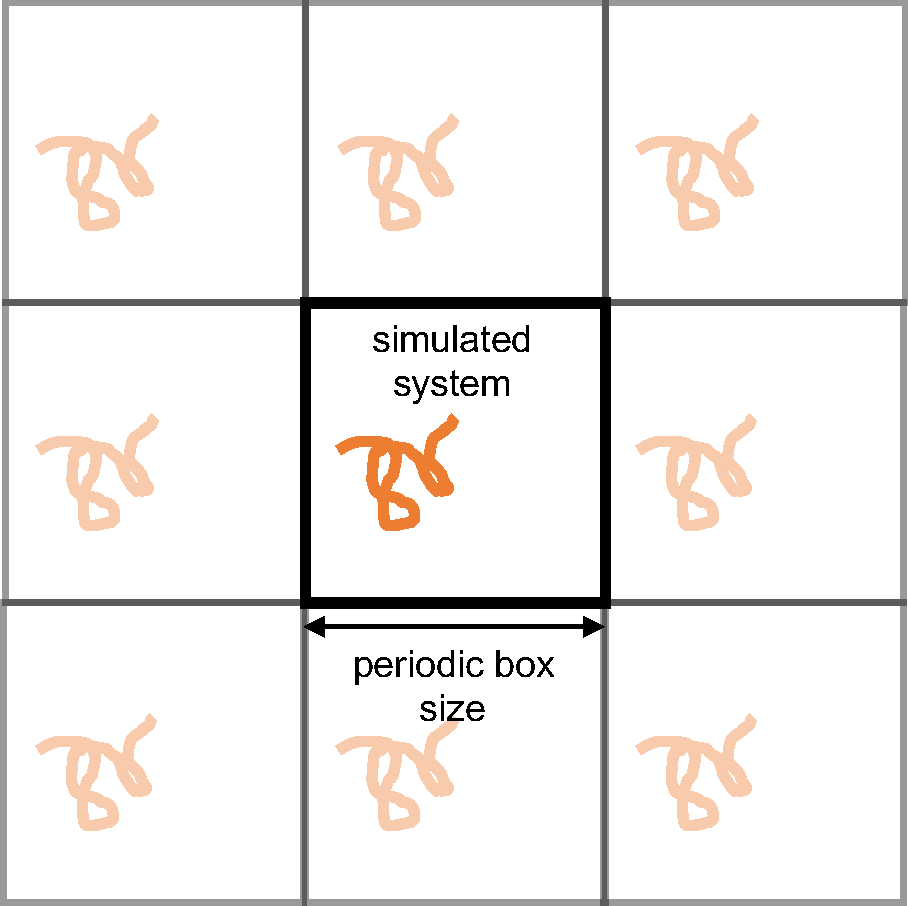
\includegraphics[width=\linewidth]{PBC_figure.pdf}
\caption{Periodic boundary conditions are shown for a simple 2D system. Note that the simulated system is a sub-ensemble within an infinitely sized system of identical, small ensembles.}
\label{pbcfig}
\end{figure}

Periodic boundary conditions allow more accurate estimation of bulk properties from simulations of finite, essentially nanoscale systems.
More precisely, simulations of comparatively small systems with periodic boundary conditions can be a good approximation to the behavior of a small subsystem in a larger bulk phase (or at least are a much better approximation than simply simulating a nanodroplet or a finite system surrounded by vacuum).
Periodic boundary conditions can alleviate many of the issues with finite size effects because each particle interacts with periodic images of particles in the same system.
Clearly, though, it is undesirable for a single particle to interact with the same particle multiple times.
To prevent this, a cut-off of many non-bonded interactions should be chosen that is less than half the length of the simulation box in any dimension.
(However, as noted in Section~\ref{sec:classical_electrostatics} these cut-offs are not normally applied to electrostatic interactions because truncating these interactions induces worse artifacts than does including interactions with multiple copies of the same particle. 
Instead, what are often termed ``cut-offs'' that are applied to electrostatics are instead a shift from short-range to long-range treatments.)
Such cut-offs impose a natural lower limit to the size of a periodic simulation box, as the box must be large enough to capture all of the most significant non-bonded interactions.
Further information on periodic boundary conditions and discussion of appropriate cut-offs may be found in \citet{LeachBook}, sections 6.5 and 6.7 and \citet{ShellNotes}, lecture on Simulations of bulk phases.
%DLM: I have permission to migrate Shell's notes to GitHub, specifically to https://github.com/kofkeLab/Mol-Sim-Intro, so I should go ahead and prioritizing these particular notes there and then cite here.

It is very important to note that periodic boundary conditions are simply an approximation to bulk behavior.
They DO NOT effectively simulate an infinitely sized simulation box, though they do reduce many otherwise egregious finite-size effects.
This is most easily seen by imagining the placement of a solute in a periodic simulation box.
The solute will be replicated in all of the surrounding periodic images.
The concentration of solute is thus exactly one per the volume of the box.
Although proper selection of non-bonded cutoffs will guarantee that these solutes do not directly interact, they may indirectly interact through their perturbation of nearby solvent.
If the solvent does not reach a bulk-like state between solutes, the simulation will still suffer from obvious finite-size effects.

Macroscopic, lab-scale systems, or bulk systems, typically consist of multiple moles of atoms/molecules and thus from a simulation perspective are effectively infinite systems.
We attempt to simulate these by simulating finite and fairly small systems, and, in a sense, the very idea that the simulation cell is not infinite, but simply periodic, immediately gives rise to finite-size effects.
Thus, our typical goal is not to remove these completely but to reduce these to levels that do not adversely impact the results of our simulations.
Finite-size effects are particularly apparent in the electrostatic components of simulations, as these forces are inherently longer ranged than dispersion forces, as discussed in Section~\ref{sec:classical_electrostatics}.
One should always check that unexpected long-range correlations (i.e. on the length-scale of the simulation box) do not exist in molecular structure, spatial position, or orientation.
It should also be recognized that periodic boundary conditions innately change the definition of the system and the properties calculated from it.
Many derivations, especially those involving transport properties, such as diffusivity \citep{Yeh2004}, assume infinite and not periodic boundary conditions. 
\todo[inline, color={green!20}]{JIM: Other examples to cite? I think there's some examples also involving calculations of entropy, but I'll have to check this}
The resulting differences in seemingly well-known expressions for computing properties of interest are often subtle, yet may have a large impact on results.
Such considerations should be kept in mind when comparing results between simulations and with experiment.

\subsection{Main steps of a molecular dynamics simulation}
\label{sec:main_steps}
While every system studied will present unique challenges and considerations,
the process of performing a molecular dynamics simulation generally follows
these steps:

\begin{enumerate}
\item System preparation
\item Minimization/Relaxation
\item Equilibration
\item Production
\end{enumerate}

Additional explanations of these steps along with procedural details specific to a given simulation package and application may be found in a variety of tutorials \citep{LemkulTutorials, AmberBeginner}.
It should be noted that these steps may be difficult to unambiguously differentiate and define in some cases.
Additionally, it is assumed that prior to performing any of these steps, an appropriate amount of deliberation has been devoted to clearly defining the system and determining the appropriate simulation techniques.

System preparation is typically the most variable of these steps, and often requires unique tools for every system of interest.
It is highly recommended that best practices documents specific to this issue and to the type of system of interest be consulted.
If such documents do not exist, considerable care should be exercised to determine best practices from the literature.
In some cases, freely available tools are constructing systems are available and can be a reasonable option (though their mention here should not be taken as an endorsement that they necessarily encapsulate best practices).
Examples include tools for constructing specific crystal structures, proteins, and lipid membranes, such as Moltemplate, Packmol, and Atomsk.
The goal of all of these tools, and system preparation in general, is to create an accurate representation of the system of interest that can be interpreted by the desired simulation package.
It is further desirable that this starting structure resemble the equilibrium structure of the system at the thermodynamic state point of interest.
For instance, highly energetically unfavorable configurations of the system, such as blatant atomic overlaps, should be avoided.
In some sense, having a good starting structure is only a convenience to reduce equilibration times (if the force field is adequate); however, for some systems, equilibration times might otherwise be prohibitively long.

System preparation is arguably the most critical stage of a simulation and in many cases receives the least attention.
Specifically, if your system preparation is flawed, such flaws may prove fatal. 
Potentially the worst possible outcome is if the prepared system is not what you intended (e.g. it contains incorrect molecules or protonation states) but is chemically valid and well described by your force field and thus proceeds without error through the remaining steps --- and in fact this is a  frequent outcome of problems in system preparation.
It should not be assumed that if a system can proceed in a well-behaved manner through the other steps, it was necessarily prepared correctly; considerable care should be taken here.

The purpose of minimization, or relaxation, is to find a local energy minimum of the starting structure so that the molecular dynamics simulation does not immediately "blow up" (i.e. the forces on any one atom are not so large that the atoms move an unreasonable distance in a single time step).
This involves standard minimization algorithms such as steepest descent.
For a more involved discussion of minimization algorithms utilized in molecular simulation, see \citet{LeachBook}, sections 5.1-5.7.

At the end of energy minimization, it is important to achieve a system configuration with small enough forces that the desired time step will allow numerical integration of the equations of motion without overly large displacements (see \citet{LeachBook}, section 7.3.4).
Such a configuration is a suitable starting point for molecular dynamics techniques.
However, this only represents a static set of positions, while the propagation of dynamics also requires a set of starting velocities.
These may be assigned in a variety of ways, but are usually randomly assigned to atoms such that the correct Maxwell-Boltzmann distribution at the desired temperature is achieved.

Following minimization, equilibration is typically needed to bring the system to the desired conditions (e.g. temperature and pressure, or energy).
Specifically, even though velocities are assigned according to the correct distribution, the selected thermostat will still usually need to add heat to or remove heat from the system as it approaches the correct partitioning of kinetic and potential energies.
For this reason, it is advised that a thermostatted simulation is performed prior to a desired production simulation, even if the production simulation will ultimately be done in the NVE ensemble.
Once the kinetic and potential energies fluctuate around constant values, the thermostat may be removed (if an NVE simulation is desired) and a snapshot selected that is simultaneously as close to the average kinetic and potential energies as possible.
This snapshot, containing both positions and velocities may be used to then start an NVE simulation that will correspond to a temperature close to that which is desired.
This is necessary due to the fact that only the average temperature is obtained through coupling to a thermostat (see Section~\ref{sec:thermostats}), and the temperature fluctuates with the kinetic energy at each time step.
Similarly, equilibration in the NPT ensemble is necessary before production in the NVT if an average density consistent with a specific pressure is desired.
In this case, the system may be scaled to the desired average volume before the production simulation.
In the above example, the NPT simulation is said to have equilibrated to a specific volume when the dimensions of the simulation box fluctuate around constant values with minimal drift. 
This definition, though not perfectly rigorous, is usually suitable for assessing the equilibration of energies, temperature, pressure, and box dimensions during equilibration simulations.
The schematic below (\ref{eqworkflow}) demonstrates what is generally an appropriate equilibriation work-flow for common production ensembles.
Clearly, this schematic cannot cover every case of interest, but should provide some idea of the general approach.
For more information on equilibration procedures, see \citet{LeachBook}, section 7.4 and \citet{ShellNotes}, lectures on Molecular dynamics and Computing properties.
%DLM: Should we be saying something here about how long to equilibrate? My short version is "until the properties of the system stop changing on average", but there could be a whole set of properties one might want to look at. Clearly you should look at anything which is important to you, but also perhaps things which tend to be relatively slow, such as water, etc.
%JIM: I tried this out above.

\todo[inline, color={yellow!20}]{DLM: Note to self, I should add a bit more discussion of what equilibration \emph{means} somewhere in this section, probably along with a discussion of equilibration vs convergence. For example, equilibration means not just that temperature and pressure stop changing but that the overall properties of teh system stop changing (e.g. if temperature and pressure is constant but your protein is unfolding you are not yet equilibrated...)}
\todo[inline, color={yellow!20}]{DLM: There are a lot of long paragraphs here that are perhaps too long; the above is one example. I should police to make sure the one-point-per-paragraph rule is used and shorten some of these.}

\begin{figure}[h]
\centering
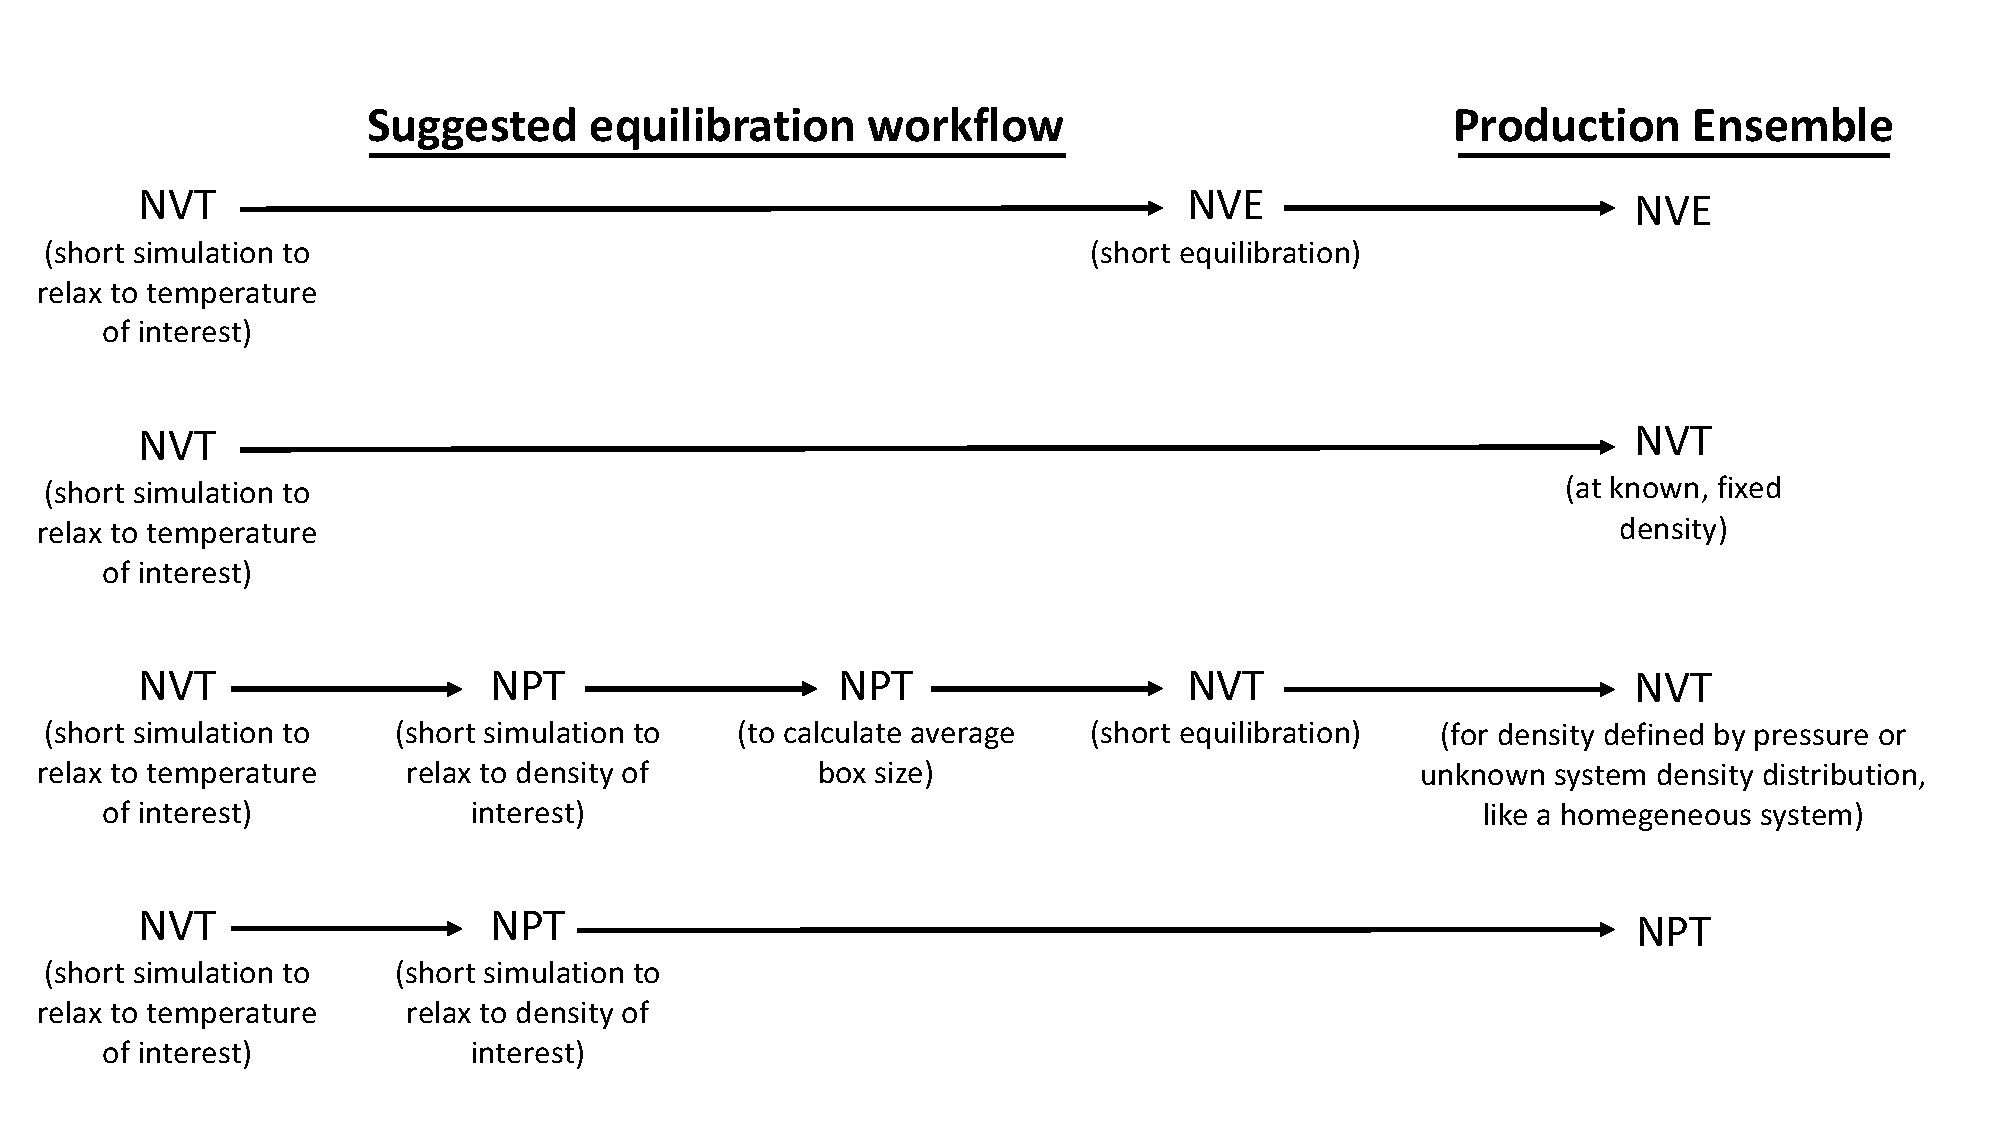
\includegraphics[width=\linewidth]{Equilibration_Workflow.pdf}
\caption{Common equilibration work-flows}
\label{eqworkflow}
\end{figure}
\todo[inline, color={yellow!20}]{DLM: Caption needs updating to make clear why you would choose different options here, especially the two different NVT options.}

Once equilibration is complete, production data may be collected.
The production simulation is that from which specific properties of the system of interest will be calculated.
As mentioned above, the equilibration procedure should be selected that is appropriate for the desired production ensemble.
It should be noted that ``equilibration'' within the production run may still be necessary before properties or metrics are computed from this simulation (see \citet{ShellNotes}, lecture on Computing Properties).
Otherwise, if a brief simulation in the same ensemble is not performed during the equilibration step immediately prior to production, any period of the production simulation should be ignored where drift is observed in the energies, temperatures, pressures, densities, or other defining state-variables of the ensemble.
This of course precedes estimation of convergence in property calculation.
Data collection then falls under the category of correctly obtaining unbiased statistics and convergence, which is covered in a separate Best Practices document (\url{https://github.com/dmzuckerman/Sampling-Uncertainty}). 
For more specific details on procedures and parameters used in production simulations, see the appropriate best practices document for the system of interest.
\todo[inline, color={yellow!20}]{DLM: Possibly clarify distinction between production and equilibration (just whether data is retained, in some cases)}

\subsection{Thermostats}
\label{sec:thermostats}

Here, we discuss why thermostats, which seek to control the temperature of a simulation, are (often) needed for molecular simulations. 
We review background information about thermostats and how they work, introduce some popular thermostats, and highlight common issues to understand and avoid when using thermostats in MD simulations.

% Motivation for using thermostats
\subsubsection{Thermostats seek to maintain a target temperature}
As mentioned above, molecular dynamics simulations are used to observe and glean properties of interest from some system of study.
However, these properties traditionally are not measurable from the initial configuration of the system, nor is that usually physically meaningful.
This generally requires transitioning the system to some other state point to collect the proper data once the system has equilibrated.
In many cases, to emulate experiments done in laboratory conditions (exposed to the surroundings), sampling from the canonical (constant-temperature) ensemble is desired\cite{thermostatAlgorithms2005}.
Generally, if the temperature of the system must be maintained during the simulation, some thermostat algorithm will be employed. 


% relevant background information needed to understand thermostats
\subsubsection{Background and How They Work}
MD simulations involve at least two kinds of temperature --- a target temperature the system should have or remain near, and an instantaneous or kinetic temperature, relating to the instantaneous properties of the system at a particular point in time.
The target temperature is the specified temperature which a thermostat is used to maintain.
However, due to the fluctuations, it is not guaranteed that the temperature measured at single point in time will be the target temperature; in reality, the instantaneous temperature \emph{should} undergo fluctuations around the target temperature.
The instantaneous temperature is also known as the kinetic temperature and is typically computed via the equipartition theorem.
It should be noted that the instantaneous temperature can be greater than, less than, or equal to the temperature corresponding to the average kinetic energy.
The kinetic temperature should also be paid special attention to when describing the system.
The kinetic temperature does \textbf{not} state ``the temperature is at some value $T$'', it merely states: ``the energy of the system is similar to that
of a system at temperature $T$''.

Several different thermostats are used to bring systems to a desired target temperature, and can be loosely grouped into three categories: deterministic, stochastic, and extended system (though some fall into multiple categories).
Deterministic thermostats are usually known to scale the momenta or forces on the particles in the system based on how consistent these are with the target temperature.
Stochastic thermostats behave similarly to the deterministic thermostats; however, they also involve a random force or momenta sampled out of a probability distribution that can that modifies the behavior of individual particles in a stochastic manner.
Extended system thermostats are similar to what their name suggests --- the system has added variable(s) and an additional degree(s) of freedom relating to the thermostat.
This emulates an external heat bath that can interact with the particles in the system, affecting their momenta in a predictable fashion.

\subsubsection{Popular Thermostats}
Within this section, various thermostats will be briefly explored, with a small description of their uses and possible issues that are associated with each.
This is by no means an exhaustive study of available thermostats; instead, we survey some of the more popular and historic thermostats used in MD.

\subparagraph{Deterministic Thermostats}
\begin{enumerate}[listparindent=\parindent]
    \item \textbf{Simple Velocity Rescaling}

        The simple velocity rescaling thermostat is one of the easiest thermostats to implement, however, this thermostat is also one of the most non-physical thermostats as well.
        This thermostat relies on rescaling the momenta of the particles every $N$ time steps based on their ratio of the instantaneous temperature to the target temperature\cite{thermostatAlgorithms2005}.
        This leads to multiple issues when trying to sample data using this thermostat.
        First, this method is not reversible, there lacks a way for the particles to have knowledge of their previous thermal history.
        This makes any dynamical value impossible to measure (diffusion for example).
        There is also no distribution of momenta; this thermostat does not sample the canonical distribution and cannot be used for sampling at thermal equilibrium.
        The isokinetic (constant kinetic energy) ensemble samples the same configurational phase space as the canonical ensemble, so position-dependent equilibrium properties can be obtained equivalently with either ensemble\cite{Minary:2003:JChemPhys:Algorithms}.
        However, the isokinetic ensemble is not properly sampled by the simple velocity rescaling thermostat, and its usage can lead to simulation artifacts, so it is not recommended\cite{Braun:2018:arXiv:Anomalous}.

    \item \textbf{Gaussian}
       % \todo[inline, color={green!20}]{EB: I recommend referring to this thermostat as the Gaussian Thermostat. I've seen it referred to as the Hoover-Evans thermostat as well (I haven't seen it called the Hoover thermostat, but I'm sure somebody has called it that), but simply calling it the Gaussian thermostat avoids wading into the argument about who came up with it first.}
        
        The goal of the Gaussian thermostat is to ensure the change in instantaneous temperature $\Delta T$ is always 0 ($\Delta T \equiv 0$); this is accomplished by modifying the force calculation with the form $F = F_{interaction} + F_{constraint}$, where $F_{interaction}$ is the standard interactions calculated during the course of the simulation and $F_{constraint}$ is a Lagrange multiplier that keeps the kinetic energy constant.
        The reasoning for the naming of this thermostat is due to the method to solve for the smallest perturbative forces needed to keep the change in temperature equal to 0.
        Using the Gaussian principle of least constraint, forces are calculated to maintain a net 0 change in temperature, while minimally perturbing the system\cite{thermostatAlgorithms2005}.
        This thermostat is reversible and it samples the isokinetic ensemble.
        Position-dependent equilibrium properties will therefore be in agreement with the canonical ensemble (as explained above), but dynamical properties will not.
        Due to the nature of the thermostat preventing a change in temperature, whatever instanteous temperature the system is at when the thermostat is applied, it will stay there. 

    \item \textbf{Berendsen}

        The Berendsen thermostat is another type of velocity rescaling thermostat, but instead of the rescaling happening very abruptly each force adjustment time, we include a relaxation term to allow the system to more slowly approach the target temperature\cite{berendsen1984molecular}.
        With the introduction of a coupling parameter $\tau$, the strength of this parameter will determine how fast the system will approach the target temperature.
        However, it should be noted that while allowing for temperature fluctuations, the Berendsen thermostat is not canonical nor is it reversible.
        Its usage can lead to simulation artifacts, so it is not recommended\cite{Braun:2018:arXiv}.

\end{enumerate}

Overall, \emph{none} of these deterministic thermostats are suitable for most production-level simulations because they do not sample from the canonical ensemble~\cite{Shirts:2013:J.Chem.TheoryComput.}, though the Gaussian thermostat has uses in some advanced applications\cite{Minary:2002:JChemPhysAlgorithms}.
The simple velocity rescaling and Berendsen thermostats can also lead to unexpected problems in systems with weak or poor coupling between degrees of freedom, such as the ``flying ice cube''~\cite{Harvey:1998:JCompChem} problem in some systems, and problems in alchemical free energy calculations where portions of the system are decoupled from the rest of the system (e.g. very rapid movement of atoms in the decoupled portion of the system); they should not be used.
To some extent, however, the choice of thermostat may depend on the property being calculated; e.g. for transport properties and kinetics, rather different issues may need consideration~\cite{Basconi:2013:J.Chem.TheoryComput.}.

\subparagraph{Stochastic Thermostats}
\begin{enumerate}[listparindent=\parindent]
    \item \textbf{Andersen}

        The Andersen\cite{andersen1980molecular} thermostat is the first of three stochastic thermostats that will be explored.
        This thermostat has vestiges of the rescaling thermostats mentioned earlier, but with a randomization element also included.  In this case, the Andersen thermostat attempts to model a system that is coupled to some random degree of freedom\cite{andersen1980molecular, thermostatAlgorithms2005}.
        In this case, this random element will be a new set of velocities that are chosen from a probability distribution and then if the reassignment probability passes, the velocities of the particle will be replaced.
        The number of particles affected, time between ``collisions'', and how often this is applied to the system are possible variations of this thermostat.
        Like the previous thermostats, this is not reversible, but the Andersen thermostat does reproduce the canonical ensemble.
        There are two versions of this thermostat, one which applies massive collisions (reassignment of all velocities) sporadically, and another which applies more gradual buffeting of selected particles.
    
    \item \textbf{Langevin}

        The Langevin\cite{schneider1978molecular} thermostat applies the idea of an implicit solvent as a way to randomly impart or remove some force acting on the particles. 
        With a general equation of the form $F = F_{interaction} + F_{friction} + F_{random}$, where $F_{interaction}$ is the standard interactions calculated during the course of the simulation, $F_{friction}$ is the damping parameter used to tune the  ``viscosity'' of the implicit bath, and $F_{random}$ is a random force perturbing the forces on the particles. 
        Careful consideration must be taken when choosing the friction damping parameter.
        However, in many cases this thermostat is an excellent option for molecular simulations.

    \item \textbf{Bussi-Donadio-Parrinello (Canonical Sampling through Velocity Rescaling)}

        The Bussi\cite{Bussi:2007:JChemPhys:Canonical} thermostat is a velocity rescaling thermostat similar to the simple velocity rescaling and Berendsen thermostats, but instead of rescaling to a single kinetic energy that corresponds to the target temperature, the rescaling is done to a kinetic energy that is stochastically chosen from the kinetic energy distribution dictated by the canonical ensemble.
        Similarly to the Berendsen thermostat, a user-specified time coupling parameter can be chosen to vary how abruptly the velocity rescaling takes place; the choice of time coupling constant does not affect structural properties, and most dynamic properties are fairly independent from the choice within a broad range.

\end{enumerate}

\subparagraph{Extended System Thermostats}
\begin{enumerate}[listparindent=\parindent]

\item {\bf Nos\'{e}-Hoover}

   The Nos\'{e}-Hoover thermostat~\cite{thermostatAlgorithms2005} essentially abstracts away the thermal bath from the previous thermostats and condenses it into a singular additional degree of freedom.
    This bath with a ``mass'' that can be changed can interact with the particles in the system in a predictable and reproducible way while maintaining the
    canonical ensemble.
    This is one of the most widely implemented and used thermostats due to these attributes.
    However, it should be noted that with small enough systems, ergodicity can be an issue and the thermostat might not properly sample the canonical ensemble \cite{martyna1992nose,thermostatAlgorithms2005}. 
    This can become important even in systems with larger numbers of particles if a portion of the system does not interact strongly with the remainder of the system, such as in alchemical free energy calculations when a solute or ligand is non-interacting.
    
    
\item {\bf Nos\'{e}-Hoover Chain}

    Briefly mentioned above, there are certain conditions where the Nos\'{e}-Hoover thermostat might not be sufficient to properly sample the system, due to
   system size and ergodicity issues\cite{martyna1992nose, thermostatAlgorithms2005}. 
    However, Martyna et al.~\cite{martyna1992nose} discovered that by coupling more heat baths to the system, the canonical ensemble can be rediscovered, at the minimal increase in computations required. In certain situations, it will be useful to chain additional heat baths to the system when under the Nos\'{e}-Hoover thermostat.

\end{enumerate}


\subsubsection{Summary}
To summarize, observe (Figure \ref{tstat_summary}), as a general summary and guide for exploring the usage of various thermostats.
Make sure to pay special attention to the reversibility when measuring time dependent properties, the ensemble sampled for all cases, and if a proper distribution of momenta and kinetic energy fluctuations are supported.
Do note that depending on the system of interest, it might not be necessary to worry about some of this information when initializing the system for a production run.
For example, if the thermal history of the system is not necessary during equilibration, a faster algorithm like Andersen or Berendsen could possibly be employed, with a switch to Nos\'{e}-Hoover for the production run.
Knowing the system you are simulating and the benefits and weaknesses to each thermostat is crucial to successfully and efficiently collect meaningful, physical data.
In general, deterministic thermostats should never be employed for production use; Langevin, Andersen, Bussi, and Nos\'{e}-Hoover chains can serve as reasonable general-purpose thermostats, and other choices should be employed only with considerable caution.

\begin{figure}[h]
\centering
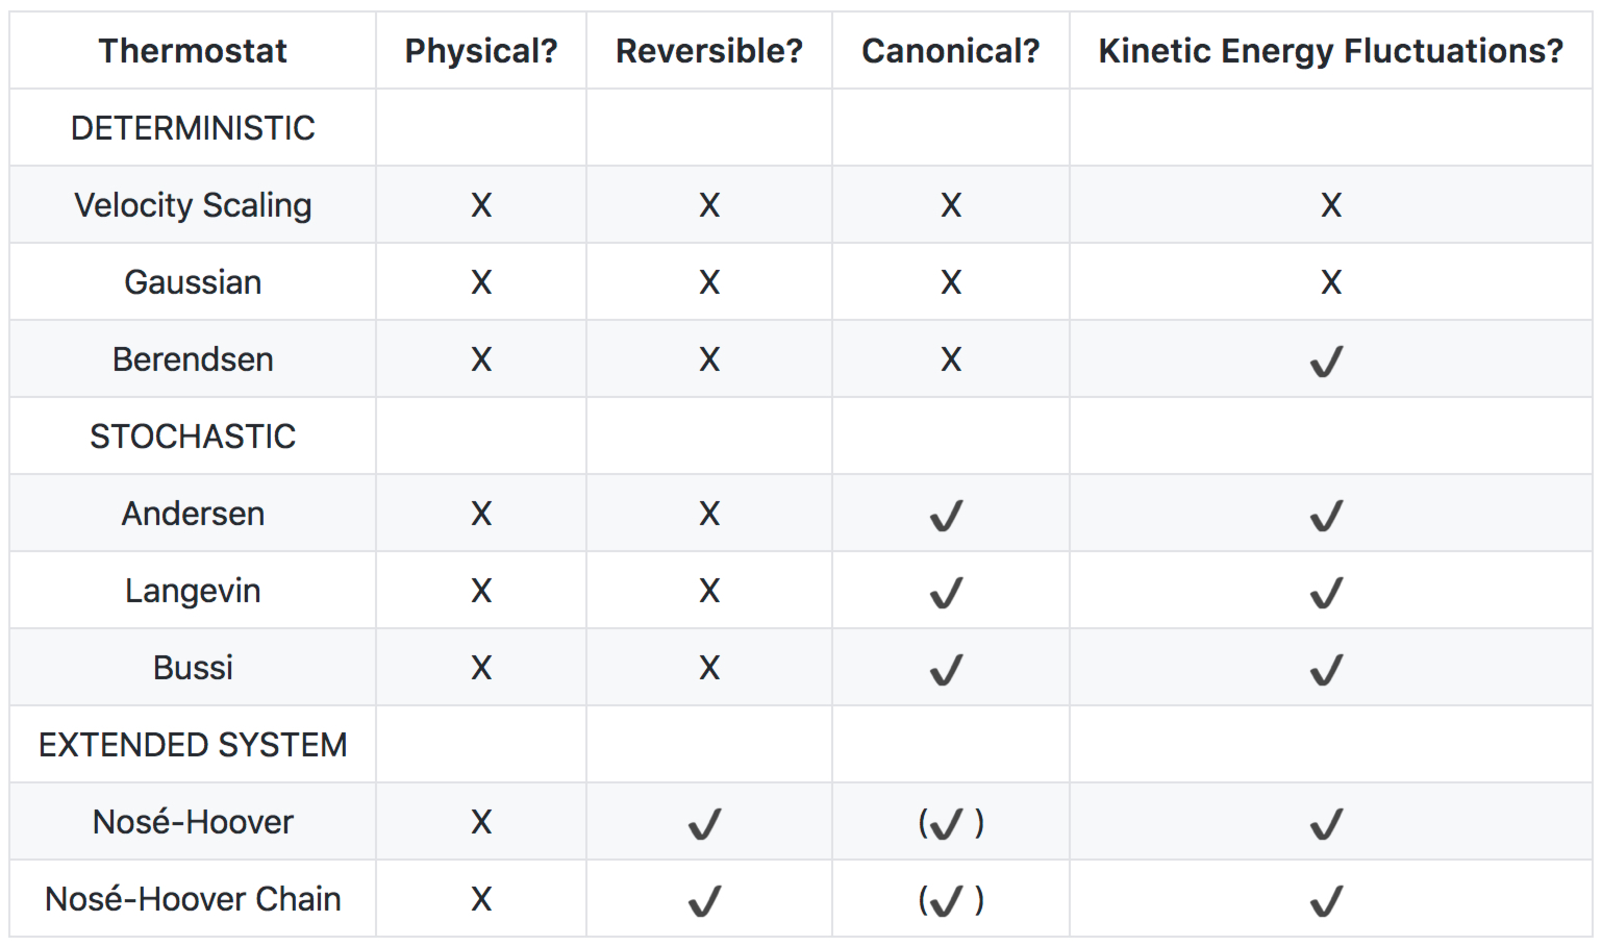
\includegraphics[width=\linewidth]{thermostat_summary.pdf}
    \caption{Basic summary of popular thermostats, where \ding{55} signifies
    that the thermostat does not fulfill that statement, \ding{51} does, and
    (\ding{51}) does under certain circumstances.}\label{tstat_summary}
\end{figure}

\subsection{Barostats}\label{sec:barostats}

Here, we discuss why barostats are used, give their background, discuss roughly how they work, describe some popular options, and summarize with some recommendations.

\subsubsection{Motivation}
Typically, thermodynamic properties of interest are measured under open air conditions in a laboratory, which (for short timescales) means at they are measured at essentially constant temperature and pressure.
Such conditions correspond to what is called the isothermal-isobaric ensemble, probably one of the most popular ensembles for MD simulationsl.
As is the case with thermostats, if the pressure must be maintained in a simulation, a barostat algorithm will be needed to sample this ensemble.

\subsubsection{Background and How They Work}
In many experiments, the container is either open to the atmosphere, meaning that it is subject to a roughly constant pressure of approximately one atmosphere. % is subjected to a constant pressure of one atmosphere; or under some enclosure, which will control the volume, thus controlling the pressure.
%DLM: Removed this; if it was sealed, it is constant volume, not constant pressure, yes?
To obtain a different pressure, some device, like a piston, inert gas, etc\@., would be needed to control the pressure and volume of the system~\cite{tuckermanBook, ShellNotes}.

For the purpose of molecular modeling, consider a hypothetical system that is being compressed and/or expanded by a fictitious piston that has some mass which acts in all directions uniformly.
Since the piston is acting on the system from all directions, it can be considered as applying a uniform compression or expansion.
The mass of the piston can be tuned to change the compression of the system, which will change how often the particles in the system will interact with the system enclosure.
These impacts from the particles on the ``enclosure'' will impart a stress on the system box which can be related to the stress the surroundings are imparting on the system.
With this relationship, we can use the virial theorem (an expectation value relating to positions and forces) to calculate the pressure of a system~\cite{ShellNotes, LeachBook}.
However, this is much more challenging when considering pairwise interactions and periodic boundary conditions~\cite{allenTildesleyLiquids, tuckermanBook, ShellNotes}, and a different approach is often utilized.
Our main point here, however, is that pressure can be related to instantaneous properties of the system allowing us to calculate an instantaneous pressure in a similar manner to how we calculate an instantaneous temperature for thermostats.

Thus, barostat algorithms apply to keep the instantaneous pressure of a system at or near the target pressure.

Barostat algorithms control pressure alone, not temperature, so if the target ensemble is isothermal-isobaric, they must also be applied with a thermostat.
If a barostat is applied without a thermostat, only the number of particles (N), the pressure (P), and the enthalpy (H) of the system is held constant.
This is known as the isoenthalpic-isobaric ensemble (NPH).
To sample from the isothermal-isobaric ensemble (NPT), a thermostating algorithm like the ones discussed earlier must also be applied.

Many barostats are available, but can usually can be classified into three main categories: volume rescaling, weakly coupled, and extended ensemble barostats~\cite{ShellNotes, tuckermanBook}. 
The next section will describe the main differences between these barostats, and give some recommendations for proper use.


\subsubsection{Popular and Notable Barostats}
Here, we introduce a few notable barostats and give a high-level summary of each, noting some key issues.
This is not an exhaustive list of barostats and barostat algorithms, just a sampling of popular and historic ones used in MD\@.

\subparagraph{Volume Rescaling}
\begin{enumerate}[listparindent=\parindent]
    \item \textbf{Volume Rescaling}

Volume rescaling barostats are the simplest example of pressure control in molecular simulations.
Every time this barostat is executed, the volume of the system is modified to produce the exact pressure desired.
This does \textbf{not} sample the proper ensemble and thus cannot be used for production sampling~\cite{ShellNotes}.
This also does not smoothly approach the target pressure either, which might cause very unphysical issues with the system during integration.

\end{enumerate}

\subparagraph{Weakly Coupled Barostats}
\begin{enumerate}[listparindent=\parindent]
\item \textbf{Berendsen}

The Berendesen~\cite{berendsen1984molecular} barostat is very similar to the Berendsen thermostat discussed earlier.
It seeks to improve upon the volume rescaling methods mentioned above.
This was to be achieved by coupling the system to a weakly interacting pressure bath~\cite{berendsen1984molecular}.
This bath scales the volume periodically by a scaling factor, which produces more realisitc fluctuations in the pressure as it slowly approaches the target pressure.
In contrast to volume rescaling, Berendsen will approach the target pressure more realistically, but the ensemble it is sampling from is not well defined and cannot be guaranteed to be NPT or NPH\@.
Berendsen can be useful for the beginning stages of equilibration, but should \textbf{not} be used for production sampling.

\end{enumerate}

\subparagraph{Extended System Barostats}
\begin{enumerate}[listparindent=\parindent]
\item \textbf{Andersen Barostat}

First described by Andersen~\cite{andersen1980molecular} in 1980, the system is coupled to a fictitious pressure bath, by adding an additional degree of freedom to the equations of motion.
This behaves as if the system is being acted upon by an isotropic piston.
This is similar to the Nos\'{e}-Hoover thermostat, which is also an extended system algorithm.
This barostat does sample the correct ensemble. However, it is isotropic in nature and applying anisotropic pressures to parts of the system is not possible.

\item \textbf{Parrinello-Rahman Barostat}

The Parrinello-Rahman~\cite{Parrinello1981} barostat is an extension to the Andersen barostat.
Unlike the Andersen barostat, Parrinello-Rahman supports the anisotropic scaling of the size and shape of the simulation box~\cite{Parrinello1981}.
This can be quite useful in solid simulations, where phase changes can be shape changes in a crystal lattice, compared to a liquid or gas, which has no well defined shape.
This barostat has essentially the same properties as the Andersen one, with the additional support anisotropy.

\item \textbf{Martyna-Tuckerman-Tobias-Klein (MTTK) Barostat}

The MTTK barostat has substantial similarity to the Parrinello-Rahman and Andersen barostats.
When Parrinello-Rahman's equations of motion were discovered to only hold true in the limit of large systems, the MTTK barostat introduced alternate equations of motion to correctly sample the ensemble for smaller systems as well~\cite{martyna1994constant, martyna1996explicit}.
Thus, MTTK~\cite{martyna1994constant, martyna1996explicit} is usually seen as an improvement over Parrinello-Rahman~\cite{Parrinello1981} for such systems.

\end{enumerate}

\subsubsection{Summary}

In summary, there are three types of barostats usually implemented in molecular dynamics codes which can greatly affect the data you are collecting from the system. 
Volume rescaling is not recommended for collection of production data.
This barostat does not sample from any correct ensemble, nor does it utilize any ``realistic'' approach to achieve the target pressure.
Weak coupling barostats provide some improvement compared to volume rescaling methods.
However, these methods cannot be used to bring the system to equilibrium effectively.
They can be used for approaching the target pressure in a more realistic fashion compared to the volume rescaling barostat, which itself is primarily useful only as a very stable thermostat for very early simulation stages if other algorithms have trouble beginning from particularly strained starting structures. 
(Alternatively, such issues can be avoided by running NVT equilibration before using a barostat, Figure~\ref{eqworkflow}.)
Finally, extended ensemble barostats are suitable for the production runs of most systems.
It is usually not recommended to use these for the equilibration process, as these barostats do not behave as well when not near the target pressure.
These can be affected by the starting configuration and pressure values much more than the Berendsen or volume rescaling barostats.
MTTK and Parinello-Rahman allow for more flexibility in terms of the shape modulation of the simulation box.
Ultimately, however, one's choice often is limited by which extended-ensemble barostat has been implemented in your simulation engine of choice.
It is recommended to begin with a volume rescaling or weakly coupled barostat to quickly bring the system to the target pressure, then switch to an extended ensemble barostat for final equilibration and production.

\subsection{Integrators}
\label{sec:integrators}

\todo[inline, color={yellow!20}]{DLM: Need to decide on ``time step'' versus ``timestep'' and change everywhere in whole paper; right now we use both.}

For systems consisting of more than three interacting bodies with no constrained degrees of freedom, there is no analytical solution to the equations of motion.
Instead, we must approximate the dynamics in a discrete manner.
This is usually termed numerical integration of the equations of motion. 
Algorithms to perform this integration take many forms and are usually called integrators.
Here, we explain the need for integrators, discuss key criteria like energy conservation, and highlight a number of commonly used integrators.

Since integration is fundamentally about taking discrete steps to approximate continuous dynamics, this discretization process introduces errors (as can be observed by comparison to analytically soluble problems, like the harmonic oscillator).
These errors are termed discretization errors, whereas additional errors called truncation errors are also accumulated through loss of precision during computer calculations.
As will be discussed shortly, there are many strategies for avoiding discretization errors.
For truncation errors, the only solution is to utilize a higher precision data type during calculations (i.e. use doubles instead of floats).

Integrators that minimize discretization error should preserve phase space volume and conserve energy.
If phase space volume is not preserved, then the sampled ensemble at a later timestep will not be the same as that in which the system was initialized.
This means that the collected data will not in fact reflect the ensemble of interest.
Luckily, this issue may be avoided simply by guaranteeing that the integrator is reversible~\cite{Frenkel:2001:}.
More details may be found in ~\citet{Tuckerman:1992:}, but basically if the mathematical operator representing the integrator preserves phase space volume, it also satisfies the definition of reversibility: if the operator is applied to propagate forward by $\Delta t$, the starting condition may be recovered by in turn applying the operator to the result using $- \Delta t$ as the timestep.

Energy conservation is imperative in simulating the microcanonical (NVE) ensemble.
This is a much trickier property to examine, and varies with different integrators.
For instance, some classes of integrators better-preserve energy over short times, while others better-preserve energy at long times.
The latter is generally preferred, though it may necessitate other sacrifices such as greater energy fluctuations away from the desired, exact system energy.
\todo[inline, color={green!20}]{JIM: Should show citations for this section where people analyze energy conservation of different integrators and make comment directing people to this. Update: I'm having trouble finding good citations here. The work is either very theoretical and involved or very old. This is really true for this entire section, so help is appreciated.}
When the energy does change over the course of a simulation, it is said to ``drift.''
The most common reason for energy drift is due to a timestep that is overly long.
If the timestep is much too long, the system can become unstable and blow up (energies become very large) due to overlap of atoms.
More subtly, the timestep may be long enough that the system is still stable over long times, but too long for the chosen integrator to conserve energy.
Other simulation parameters may also impact energy drift, such as the method of truncating forces and energies, as well as the choice of numerical precision.
The latter effect, due to truncation errors, will become obvious if two simulations with different timesteps are compared.
Shorter timesteps, and hence more steps to achieve a simulation of the same length, will result in \textit{more} drift, since errors get larger with the number of calculations performed by the computer.
This is exactly opposite to the behavior that is expected for poor energy conservation associated with discretization error, where a shorter timestep will reduce energy drift.
\todo[inline, color={yellow!20}]{DLM: Probably need to address energy drift, as well as how energy changes should scale with timestep.}
\todo[inline, color={green!20}]{JIM: I addressed some of this above. I'm not sure exactly about the scalings, though. Can you say for sure how energy drift scales with timestep or number of timesteps?  Isn't this highly algorithm-specific (and maybe even system-specific)?}

Additionally, it is also desirable that an integrator be computationally efficient.
Integrator cost mostly appears in the length of the timestep that may be taken while still avoiding discretization error. 
As discussed further below, the timestep must be at least an order of magnitude less than the smallest timescale of motion present in the system.
However, depending on the accuracy of the integrator with respect to reproducing the true dynamics, a smaller timestep might be necessary.
If the integrator requires a very small timestep to avoid discretization error, then the computational cost greatly increases.
Hence, a truly ``good'' integrator allows for long timesteps while still achieving low discretization error.
This has the added benefit of also reducing truncation error, which is proportional to the number of timesteps taken.
It is worth noting that the issue of integrator choice versus timestep is not always simple; in some cases, a ``better'' integrator might allow longer timesteps but also carry an additional computational cost that outweighs the benefits of an increased timestep.

The most commonly used integrators are variants of the Verlet algorithm (e.g. Velocity Verlet or Leapfrog). 
Detailed discussion and derivation of such integrators may be found in section 7.3 of \citet{LeachBook} and 4.3 of \citet{Frenkel:2001:}.
Such integrators are not applicable, however, for simulations involving stochastic dynamics.
These simulations include application of a random force to each particle, and represent discretizations of either Langevin or Brownian dynamics.
A detailed description of such stochastic dynamics may be found in McQuarrie~\cite{McQuarrieStatMechBook}, Chapter 20.
As detailed in section \ref{sec:thermostats}, it is common to apply temperature control through the use of Langevin dynamics.
As a brief aside, this highlights the fact that the choice of integrator is often tightly coupled to the choice of thermostat and/or barostat.
Different combinations may demonstrate better performance and for expanded ensemble methods it is absolutely necessary to utilize an integrator specific to the selected temperature- or pressure-control algorithm.
For simulating Langevin or other stochastic dynamics, the presence of random forces usually prevents the integrator from preserving phase-space volume.
However, through fortuitous cancellation of error, some stochastic integration schemes may achieve preservation of \textit{part} of the full phase-space (i.e. configurations \textit{or} velocities are preserved)~\cite{Fass2018}.
Though this may sound dire, in practice this is easily remedied through an appropriate choice of timestep - this just might need to be shorter or longer depending on the integration scheme.
When using Langevin or Brownian dynamics, one should also be aware that calculations of any dynamic properties with longer timescales than the application of the random forces will be very different than those from deterministic trajectories.
If one is only interested in configurational or thermodynamic properties of the system, this is of no consequence.
If dynamics are of interest, the dependence of these properties on the integrator parameters (e.g. friction factor) should be assessed~\cite{Basconi:2013:J.Chem.TheoryComput.}.
\todo[inline, color={yellow!20}]{DLM: I need to review the paragraphing here; some of these are rather long and cover a lot. }

\todo[inline, color={green!20}]{JIM: Happy to introduce Trotter decompositions, but is it really necessary? Also, we need to add information on constrained dynamics.  Anything else?  Needs more details, or just send people to citations?}
\todo[inline, color={yellow!20}]{DLM: I don't think necessary to introduce, but in favor of adding citations to useful work/additional resources.}

\subsubsection{How to choose an appropriate timestep?}
\todo[inline, color={yellow!20}]{DLM: Above should be broken into subsubsections for consistency with thermostats/barostats and because a subsection with only one subsubsection doesn't make sense.}

The maximum timestep for a molecular dynamics simulation is dependent on the choice of integrator and the assumptions used in the integrator's derivation.
For the commonly-used second order integrators such as the Verlet and Leapfrog algorithms, the velocities and accelerations should be approximately constant over the timestep.
Thus, the timestep is limited by the highest frequency motion present in the system, which for all-atom simulations is usually bond vibrations.
It is commonly found that using a timestep that is one tenth of this vibration's characteristic period is sufficient to conserve energy in the microcanonical ensemble.
For example, if hydrogen molecules are present in the simulation box and the H-H bond vibration is the highest-frequency motion in the system, one can determine that with a force field harmonic force constant of approximately 500 N/m, the oscillation period will be 8 fs; thus, a 0.5 fs timestep can be used.
For all-atom simulations with constraints on the high-frequency bonds, timesteps can be commonly increased to 2 fs; coarse-grained simulations with particles of higher mass and smaller force constants can have much larger timesteps.
After choosing a timestep, a test simulation should be run in the microcanonical ensemble to ensure that the choice of timestep yields dynamics that conserve energy.
Methods also exist to increase the timestep beyond the limit imposed by the system's highest-frequency motion.
Many such enhanced timestepping algorithms exist such as multiple-timestep methods which separately integrate high-frequency and low-frequency motion and schemes which repartition atomic masses to decrease the highest-frequency motion seen in the system\cite{Berne:1999:Molecular,Hopkins:2015:JCTC:Long}.


\subsection{Long range electrostatics}
\todo[inline, color={yellow!20}]{DLM: I need to edit this section after we get Samarjeet's changes in; skipping for now.}
\label{sec:lr_electrostatics}
\begin{itemize}
\item Cut-off is bad
\item Need for special treatment
\item Idea of an Ewald sum
\item PPPM
\item How to choose parameters
\end{itemize}


\subsubsection{Motivation}

Calculation of non-bonded interaction is generally the most time-consuming step of classical energy calculation. While the elements(?) for bonded interaction remain unchanged during the course of MD simulation, the ones for non-bonded interactions have to be updated frequently. Furthermore, $r^{-1} $ dependence  of coulombic interaction in a 3D space complicates the calculation in the following two ways :
\begin{itemize}
\item Coulombic potential is conditionally convergent. What do we mean by this? Consider for example the alternating harmonic series : \\
\[
\sum_{k=1}^{\infty} \frac{-1^{k+1}}{k} = 1 - \frac{1}{2} + \frac{1}{3} - \frac{1}{4} + \frac{1}{5} - ... = ln 2 
\]

But if we now change the order of the summation to, lets say :
\[
( 1 - \frac{1}{2})  - \frac{1}{4} + (\frac{1}{3} - \frac{1}{6}) - \frac{1}{8} + (\frac{1}{5} - \frac{1}{10}) - \frac{1}{12} + (\frac{1}{7} - \frac{1}{14}) - \frac{1}{16} + .. 
\]
\[
= \frac{1}{2} - \frac{1}{4} + \frac{1}{6} - \frac{1}{8} + \frac{1}{10} - ... 
\]
\[
= \frac{1}{2} (1 - \frac{1}{2} + \frac{1}{3} - \frac{1}{4} + \frac{1}{5} - ...) = \frac{1}{2} ln 2
\]

Using a different order might give us a different result. Thus the order of summation matters !

\item Coulombic potential is a slow-decaying, long range potential. This means that we need to account for non-bonded pairs over larger pairwise distances in order to minimize the errors. As enlisting atom-pairs is fundamentally an $O(n^2) $ operation, the time taken to compute non-bonded pairs increases quadratically with respect to an increase in the number of atoms.   
\end{itemize} 

As discussed earlier, simulations are generally performed under periodic boundary conditions, i.e. potential at any point is due to all the other charges in the system as well as their infinite images. Hence different methods have been developed to optimize the electrostatic potential. An obsolete method is to just use spherical truncation, i.e. only consider the interactions within a cutoff distance $(r_c)$. This method has been shown to suffer from the following artifact : Consider the radius-rc sphere around a particle. In general, this sphere would be charged as exactly same number of positive and negative charges would be required to make it neutral. During the course of dynamics, charged particles can move back and forth the boundary at $r_c$, thus creating an artificial effect due the boundary(ref: Allen and Teldsley).  

\subsubsection{ Ewald Summation}

One way of handling the aforementioned issues in an efficient manner is to use the Ewald summation technique (ref, Ewald 1921). To understand this technique, lets represent the relation between the charge distriution and the coulombic potential  in the differntial form (Poisson equation) :

\[
\Delta \phi(\boldsymbol{x}) = - \frac{1}{\epsilon} \rho(\boldsymbol{x}) 
\] 

where,  $ \boldsymbol{x} \epsilon R^3 $ ,  $\phi(\boldsymbol{x})$ is the potential at point $\boldsymbol{x}$, $\rho(\boldsymbol{x})$ is the charge at point $\boldsymbol{x}$ and $\epsilon$ is the permissivity of the medium. This equation is an elliptical partial differential equation(pde) of the second order. The standard way to determine the potential from this equation is a two step method - discretization of the equation followed by solution. These techniques however depend on the smoothness of the functions - $\rho$ and $\phi$ - involved. However, in the case of charge distribution in our simulation system, $\rho$ is a set of delta functions which are clearly not smooth! As $\rho$ is not smooth, $\phi$ is not smooth either. \\

   
Ewald method is based on replacing the point charge distributions by smooth charge distributions in order to use the fast solvation techniques of the pde. The most common smooth function used in Ewald method is the gaussian distribution although other distributions have been used as well. Thus,

\[ \rho = \rho^{sr} + \rho^{lr} \]

\[ \rho^{sr} = q\delta(\boldsymbol{x}-\boldsymbol{x_i}) - qG\] 

\[ \rho^{lr} = qG \]      


\begin{figure}[h]
\centering
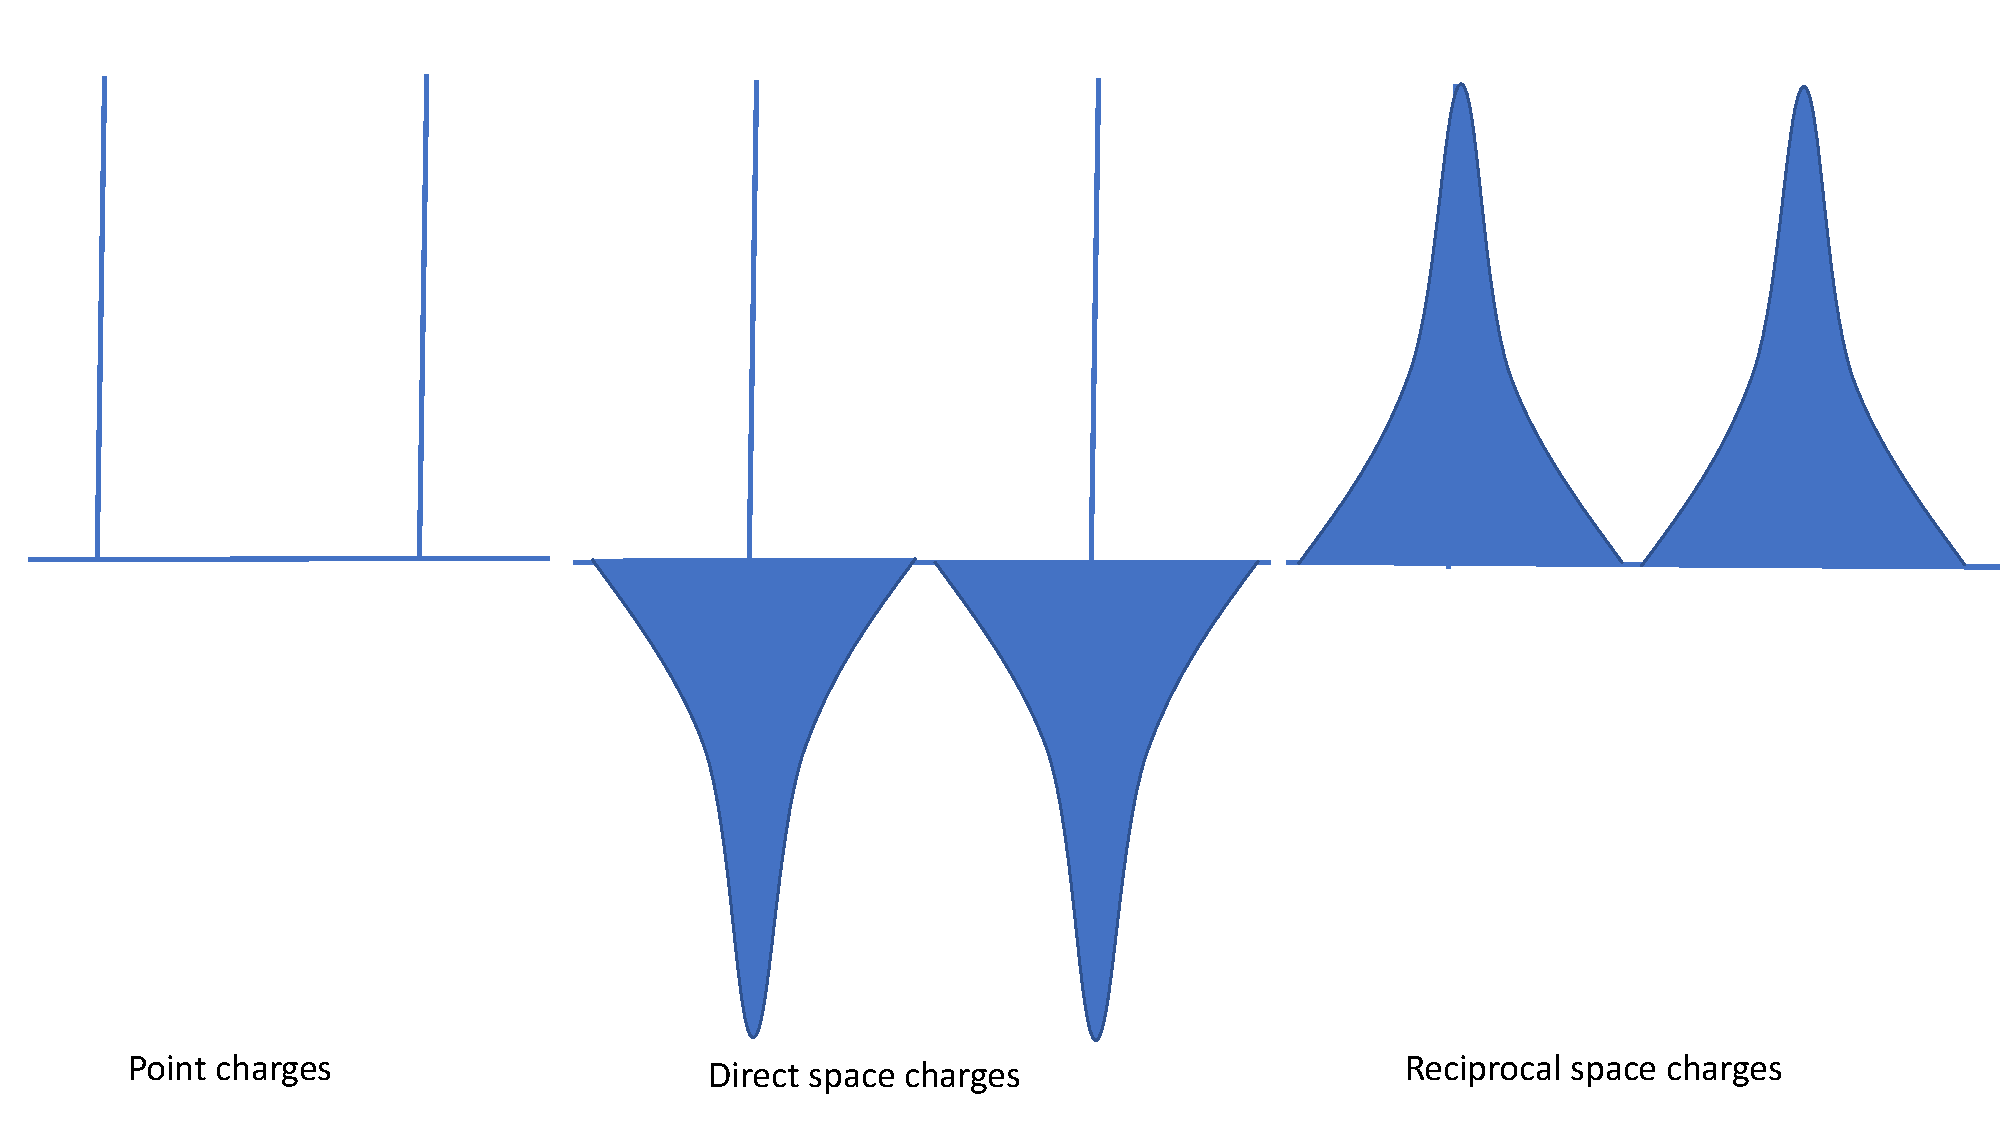
\includegraphics[width=\linewidth]{charges_ewald.pdf}
    \caption{Point charges can be split into Direct space and reciprocal space charges. Direct space charge consists of the original charges and gaussian-distributed screening charge. Reciprocal space charge is only the gaussian-distributed charge.}
\label{charges_ewald}
\end{figure}

Direct space or short range charge ($\rho^{sr}$) consists of the original point charge screened by the gaussian-distributed charge of the same magnitude. 
\[
E^{sr} = \frac{1}{2} \sum_{n \in Z^3}^{'} \sum_{i,j}q_i q_j \frac{erfc(\alpha|r_{ij} + nL|}{|r_{ij} + nL|}
\]

Unlike the potential due to the original charge, the potential due to direct space charge decays rapidly as shown in the figure. This is due to erfc function which decays very fast. Infact, it decays even faster than the Van der Waals term $r^{-6}$ and hence the cutoff used for Van der Waals can be used for direct space coulombic potential calculation as well. 

Potential due to the long range charge however doesn't decay rapidly and if calculated in the direct space would require summation over the infinite images. However, as we discussed earlier, the smoothness of the  charge $\rho^{lr}$ (and hence potential ($\phi^{lr}$) allows the use of fast pde solvers. Fourier based solvers use the important result that differentiation operation in direct space corresponds to multiplication by (ik) in reciprocal space! 

\[
E^{lr} = \frac{1}{2L^3} \sum_{k \neq 0} \frac{4\pi}{k^2} \exp^{-\frac{k^2}{4\alpha^2}} |\rho(k)|^2
\]

The interesting factor here in $E^{lr}$ is the $\exp (-k^2)$ which decays exponentially. If we used only the original point charges, we would not have had this dampening factor. 

Self term is not a physical quantity and comes up due to the way the Ewald summation is set up. 

\[
E^{s} = - \frac{\alpha}{\sqrt{\pi}}\sum_i q_i^2
\]
 
\subsubsection{Grid based Ewald summation}

Ewald summation, through Fourier transform, as described in the previous section takes $O(n^{3/2})$ time. Discrete Fourier Transform (DFT) provides a  faster way of solving the problem and reduces the time complexity to $O(n log(n))$. In order to use DFT, the charge distribution has to be discretized over a grid. Particle-Particle Particle Mesh (P3M), Particle Mesh Ewald (PME) and Smooth Particle Mesh Ewald (SPME) are three different implementations of the grid-based solution and are very similar in spirit though the details are slightly different. The choice of specifics in each one is based on a combination of accuracy, speed and ease of implementation. In this subsection, we give an overview of the grid-based approach. 

There are five general steps involved in these methods :
\begin{enumerate}
\item Charge assignment : In this step, charges are interpolated onto the grid. While the original PME method uses Lagrangian interpolation for charge assignment, the SPME method uses the smoother cardinal B-splines of order n ($M_n$).  

\[
Q(k_1,k_2,k_3) = \sum_{i=0}^{N}\sum_{p_a=0}^{K_a-1} q_i \prod_{d=1}^3 M_n(u_i^d - k_d - p_dK_d)
\]
\item Transformation of the grid to reciprocal space : Fast Fourier Transform (FFT) is used to convert the charges on the grid to their equivalent fourier space structure factors.    
\[
S(m) = \sum_j q_j \exp(mr_j)
\]
\[
=\prod_{i=1}^{3} b_i(m_i)F(Q)(m_1,m_2,m_3)
\]
where
\[
b_i(m_i) = \exp(2\pi i (n-1)m_iK_i) X
\]
\[ [\sum_{k=0}^{n-2}M_n(m+1)\exp{2\pi im_ik/Ki}]^{-1}
\] 
\item Energy calculation : Reciprocal space energy is calculated by
\[
E^{rec} = \frac{1}{2} \sum_{m_a=1}^{K_a-1} Q(m_1,m_2,m_3)(\theta_{rec}*Q)(m_1,m_2,m_3)
\]
where
\[
\theta_{rec} = F(BXC)
\]

\[
B(m_1,m_2,m_3) = \prod_{i=1}^{3} |b_i(m_i)|^2
\]
and
\[
C(m_1,m_2,m_3) = \frac{1}{\pi V} \frac{ \exp{- \pi^2 m^2 \beta^2}}{m^2}
\]
Here * is the convolution operation which is simply a product in the reciprocal space. 
\item Transformation of the grid back to real space : Inverse FFT is used to convert $\theta{rec}*Q$ back to the real space. 
\item Force calculation : Force is given by the gradient of the energy. It can be calculated in the reciprocal space by multiplication by (ik) (as implemented in the original PME) or by analytic differentiation in the real space as in SPME : 
\[
\frac{\delta E_{rec}}{\delta r_i^a}  = \sum_{m_a=0}^{K_a-1} \frac{\delta Q_{rec}}{\delta r_i^a}(m_1,m_2,m_3) (\theta_{rec}*Q)(m_1,m_2,m_3)
\]
\end{enumerate}



Optimizing the performance of grid based methods is tricky as many of the choices would already have been made in the implementation of the method. As a user, there are a few ways to tweak the performance of the SPME : 
 
\begin{itemize}
\item Grid dimensions : A fine grid would be slower as the interpolation and calculations would have to be done at larger number of points. However its accuracy will be higher than a coarse grid.
\item Screening function : Some variants of Ewald summation have used screening function other than  gaussian. In SPME implementations, one uses the Gaussian. The screening function can be varied via the spread of the gaussian.  However, as discussed earlier, it is tightly coupled with direct space cutoff.
\item Cutoff of the direct space : Although it can be changed, it is generally kept the same as van der waals cutoff for the ease of implementation. Decreasing the cutoff improves the direct space performance but increases the complexity of the reciprocal space calculations. 
\end{itemize}


\todo[inline, color={yellow!20}]{DLM: Need to write some kind of wrap-up/conclusion rather than just ending abruptly. Also probably should mention again data analysis and point to Zuckerman work. }
\todo[inline, color={yellow!20}]{DLM: Perhaps also a brief ``what NOT to do with your MD data'' blurb, e.g., don't just make movies and look at them. Don't treat them as the answer. Don't overinterpret, etc.}
\todo[inline, color={yellow!20}]{DLM: Also need to point out the checklist below and discuss it in the text somewhere.}
\todo[inline, color={yellow!20}]{DLM: I also need to go over the checklist again and make sure it is what we want/addresses key issues (and everything there is addressed in the text.}

%\subsubsection{Other methods}

%There are methods other than the Ewald which we can use as well 
%\begin{itemize}
%\item Isotropic periodic sum It doesn't use the Ewald
%\item Multigrid method It doesn't use Fourier 
%\end{itemize}

\begin{Checklists*}[p!]

\begin{checklist}{Take stock of your plans}

\begin{itemize}
\item \textbf{Count the cost: } Think about what you know about the timescales of what you want to observe and determine whether it is tractable to simulate this given the size of your system, your computational resources, and the expense of the simulation.
\item Pick the desired ensemble ($NVT$, $NPT$, $NVE$, $\mu VT$, $\mu PT$)
\item Determine reference states that you are trying to emulate/discover.
\item What temperature, pressure, etc. are you interested in?
\item What is already known in the literature and what data do you wish to compare to?
\end{itemize}
\end{checklist}

\begin{checklist}{Prepare to implement your plans and make critical decisions about system type}

\begin{itemize}
\item Choose a simulation package suitable for simulating that ensemble (see best practices document) % link
\item Determine whether you are simulating a bulk (typically periodic) or finite system and choose the appropriate cutoff types and periodicity (full periodicity for bulk systems, partial periodicity for interfaces, etc.) as discussed in [section] % reference section whatever
\end{itemize}
\end{checklist}

\begin{checklist}{Determine handling of cutoffs}
\begin{itemize}
\item As a general rule, electrostatics are long-range enough that either the cutoff needs to be larger than the system size (for finite systems) or
periodicity is needed 
\item Nonpolar interactions can often be safely treated with cutoffs of 1-1.5 nm as long as the system size is at least twice that, but long-range dispersion corrections may be needed
\end{itemize}
\end{checklist}

\begin{checklist}{Choose appropriate settings for the desired ensemble:}
\begin{itemize}
\item Pick a thermostat that gives the correct distribution of temperatures, not just the correct average temperature
\item Pick a barostat that gives the correct distribution of pressures
\item Consider the known shortcomings and limitations of certain integrators and thermostats/barostats and whether your choices will impact the properties you are calculating
\end{itemize}
\end{checklist}


\begin{checklist}{Choose an appropriate timestep for stability and avoiding energy drift}
\begin{itemize}
\item This depends on factors such as the use of constraints in the system (e.g. for all-atom systems constraining hydrogen bonds can allow the use of a slightly longer timestep; 2 fs is relatively typical)
\end{itemize}
\end{checklist}


\end{Checklists*}







\nocite{*}
\bibliography{basic_training}{}

\end{document}
